\chapter{Simulation du cas d'une goutte avec transfert de masse : comparaison qualitative à une expérience de la littérature}

Dans cette partie, on s'intéresse à la simulation d'une expérience de la littérature où une goutte soumise à un transfert de masse avec la phase continue dans laquelle elle est plongée monte puis redescend. De par les limitations actuelles du modèle en développement dans TrioCFD qui seront précisées dans ce chapitre, la comparaison à l'expérience ne sera que qualitative et le travail portera principalement sur le paramétrage du modèle et l'évaluation (au travers d'une étude paramétrique) de l'influence de divers paramètres.


\section{Présentation de l'expérience et des résultats rapportés dans Rao et al.  \cite{rao_influence_2015}} \label{sec:presExp}
L'objectif de l'expérience présentée par Rao et al. est d'étudier expérimentalement l'influence de la diffusion massique sur la trajectoire goutte soumise à la gravité. Cette goutte est initialement composée d'acétonitrile (miscible dans l'eau) et de chlorobenzène (immiscible) dans de l'eau. La goutte est formée de telle sorte que sa masse volumique soit inférieure à celle de l'eau créant un mouvement ascendant de la goutte. La diffusion de l'acétonitrile dans l'eau va alors provoquer l'augmentation de la masse volumique de la goutte jusqu'à la redescente de celle-ci. Le schéma de l'installation expérimentale est présenté en Figure \ref{fig:exp}.
\begin{figure}[H]
	\centering
	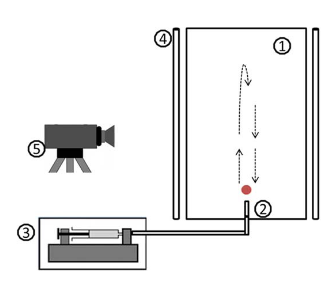
\includegraphics[width=0.3\linewidth]{figure/exp}
	\caption{Schéma de l'installation expérimentale, d'après \cite{rao_influence_2015}}
	\label{fig:exp}
\end{figure}
L'article présente également un modèle \textit{CFD} qui calcule le transfert de masse semi-empiriquement. Ce modèle propose une résolution 2D axisymétrique des équations de Navier-Stokes avec une capture d'interface de type VOF (\textit{Volume of fluid}) et une reconstruction linéaire de l'interface (PLIC). L'équation de suivi de l'évolution de la fraction massique d'acétonitrile contient un terme source quantifiant le transfert de masse entre les deux phases au travers d'un coefficient d'échange massique. Ce coefficient est obtenu à l'aide de corrélation en faisant l'hypothèse d'une goutte sphérique. L'objectif est de réaliser qualitativement sur TrioCFD le cas n$^\circ$ 4 de l'article. Les principaux paramètres de l'étude sont rassemblés dans le Tableau \ref{table:rao_al}.

\begin{table}[H]
	\centering  % not needed, since table is as wide as text block
	\begin{tabularx}{\textwidth}{@{}lYYYYYYY@{}}
		\toprule
		&\multicolumn{6}{c}{}\\
		%\cmidrule(lr){2-3} \cmidrule(l){4-5} 
		& $L_x$ (m)
		& $L_y$ (m)
		& $dx, dy$ (m)
		& Nombre de maille
		& $\rho^{drop,init}$ (kg.m$^{-3}$)
		& Concent. init. acétonitrile
		& $D^{drop}$  (m)\\
		\midrule
		 Valeurs & 15.$R^{drop}$ & 60.$R^{drop}$ & 4,08.10$^{-6}$ 1,85.10$^{-6}$ 1,65.10$^{-6}$ & 40.10$^{3}$  \hspace{2cm}  72.10$^{3}$  \hspace{2cm} 81,6.10$^{3}$ & 975 & 0,32& 4,9.10$^{-3}$ \\
		\bottomrule
	\end{tabularx}
	\caption{Paramètres des simulations CFD, d'après Rao et al.\cite{rao_influence_2015}} \label{table:rao_al}
\end{table}
Les paramètres de résolution de maillage ($dx,dy$) correspondent aux valeurs minimales de ces paramètres, le maillage étant raffiné au niveau de la goutte. Les résultats de l'article considèrent un temps initial correspondant à la seconde suivant la formation de la goutte. Ainsi, il existe une forte incertitude sur les conditions initiales de vitesse ainsi que sur la concentration. En effet, dès l'instant où la goutte est formée, le transfert de masse opère entre la goutte et l'eau. Pour la suite de ce travail nous considérons donc une vitesse initiale nulle ainsi que des concentrations initiales tels qu'elles nous sont données. Dans la suite de ce chapitre, nous considérons deux phases, l'une dispersée (notée $disp$) et l'autre continue (notée $cont$), de plus les éléments seront notés miscible ($misc$) pour l'acétonitrile et immiscible ($immi$) pour le chlorobenzène.
Finalement, la suite de ce chapitre consistera en la comparaison entre les résultats obtenus via TrioCFD en utilisant une description analytique de l'énergie et ceux présentés par Rao et al. \cite{rao_influence_2015}.
%\begin{figure}[H]
%	\centering
%	\small
%	\begin{tikzpicture}[scale=0.75, transform shape]
%	\node[draw,aspect=1.3, text centered,text width=3cm] (V) at (0,2.3) {Solution initiale };
%	\node[draw,aspect=1.3, text centered,text width=2cm] (T) at (0,1.3) {$n=n+1$ };
%	\node[draw,rectangle, text centered,minimum width=2cm,minimum height=1cm] (A)at(0,0){Estimation du transfert de masse à partir de corrélations};
%	\node[draw,text centered,minimum width=2cm,minimum height=1cm] (B) at (0,-1.5) {Résolution des équations de Navier-Stokes};
%	\node[draw,text centered,text width=10cm,minimum height=1cm] (C) at (0,-3) {Comparaison entre l'altitude de la goutte obtenue par CFD avec l'expérience, res = $f(z_{\text{CFD}},z_{\text{exp}})$};
%	\node[draw,rectangle,diamond, aspect=1.3, text centered,text width=1.5cm] (D) at (0,-5) {res $<\varepsilon$ ? };
%	
%	\node[draw,rectangle,diamond, aspect=1.3, text centered,text width=1.5cm] (E) at (0,-7.3
%	) { $t^{f}<t^{n}$ ? };
%	\node[draw,aspect=1.3, text centered,text width=1.5cm] (W) at (0,-9) {Fin};
%	%\node[draw,text centered,text width=2cm,minimum height=1cm] (E) at (0,-6.8) { $t=t^{n+1}$};
%	%\node[draw,text centered,text width=7cm,minimum height=1cm] (Z) at (0,-6.2) { dsq}
%	
%	\node[draw,rectangle,diamond, aspect=1.3, text centered,text width=1cm,color=white] (H)at(-5,-5.9){ };
%	\node[text centered,text width=1cm,color=black] (K1)at(0.5,-5.9){oui};
%	\node[text centered,text width=1cm,color=black] (K2)at(-1.5,-4.8){non};
%	\node[text centered,text width=1cm,color=black] (K3)at(0.5,-8.3){oui};
%	\node[text centered,text width=1cm,color=black] (K4)at(-1.5,-7){non};
%	%\node[draw,rectangle, text centered,diamond, aspect=1.3, text centered,text width=1cm] (I)at(6,-6){i=1 to n-1};
%	\draw[->] (T.south) -- (A.north);
%	\draw[->] (A.south) -- (B.north);
%	\draw[->] (B.south) -- (C.north);
%	\draw[->] (C.south) -- (D.north);
%	\draw[->] (D.south) -- (E.north);
%	\draw[->] (V.south) -- (T.north);
%	\draw[->] (E.south) -- (W.north);
%	\draw[->] (-7,1.3) -- (T.west);
%	
%	
%	
%	\draw (D.west)-- (-6,-5);
%	\draw (-6,-5)-- (-6.,0);
%	%	\draw (F.west)-- (-6.,0);
%	\draw[->] (-6.,0) -- (A.west);
%	\draw[-] (E.west) -- (-7,-7.3);
%	\draw[-] (-7,-7.3) -- (-7,1.3);
%	%\draw (G.east)-| (I.south);
%	%\draw[->] (I.north)|- (A.east);
%	\end{tikzpicture}
%	\caption{Algorithme de résolution développé par Rao et al.\cite{rao_influence_2015}}
%	\label{fig:algoRao}
%\end{figure}
\section{Conditions initiales} \label{sec:difficulte}
Au cours de cette étude, on distingue plusieurs types de simulations, les premières étant réalisées sans couplage avec les équations de Navier-Stokes pour vérifier le comportement de la goutte et la cohérence du paysage thermodynamique. Dans un second temps, des simulations avec couplage seront réalisées. Les conditions initiales de concentration s'écrivent sous la forme :
\begin{equation}
\phi_{i}(\mathbf{x},t=0) = \frac{\phi^{init,cont}_i + \phi^{init,disp}_i  }{2} +  \frac{\phi^{init,cont}_i - \phi^{init,disp}_i }{2}\tanh\left(\cfrac{\sqrt{(x-x_0)^2+(y-y_0)^2}-R}{\epsilon} \right)
\end{equation}
Avec ($x_0$, $y_0$) les coordonnées du centre de la goutte, $R$ le rayon de la goutte, $\epsilon$ l'épaisseur de l'interface et $\phi_i^{init,cont}$ (resp. $\phi_i^{init,disp}$) la concentration initiale de l'élément $i$ dans la phase continue (resp. dispersée). Les valeurs initiales du paramètre d'ordre sont calculées telles que :
\begin{subequations}
	\begin{empheq}[left={\empheqlbrace\,}]{align}
	&\phi_{misc}^{init,disp} =  \frac{1}{\beta_{misc} - \beta_{immi}} \left( \frac{\rho^{init,disp}}{\rho_{eau}} - \beta_{immi} -1 \right) \\
	%1 / (beta1Boussinesq - beta2Boussinesq) * ((rhoInitialDroplet / rhoWater) - beta2Boussinesq - 1)
	&\phi_{immi}^{init,disp} = 1 - \phi_{misc}^{init,disp}
	\end{empheq}
\end{subequations}
\noindent Avec $\rho^{init,disp}$ la masse volumique initiale de la goutte, $\beta_{k}$ le coefficient de dilation associé au composant $k\{misc,immi\}$, un exemple de condition initiale est donné en Figure \ref{fig:conditioninit}.
\begin{figure}[H] 
	\centering
	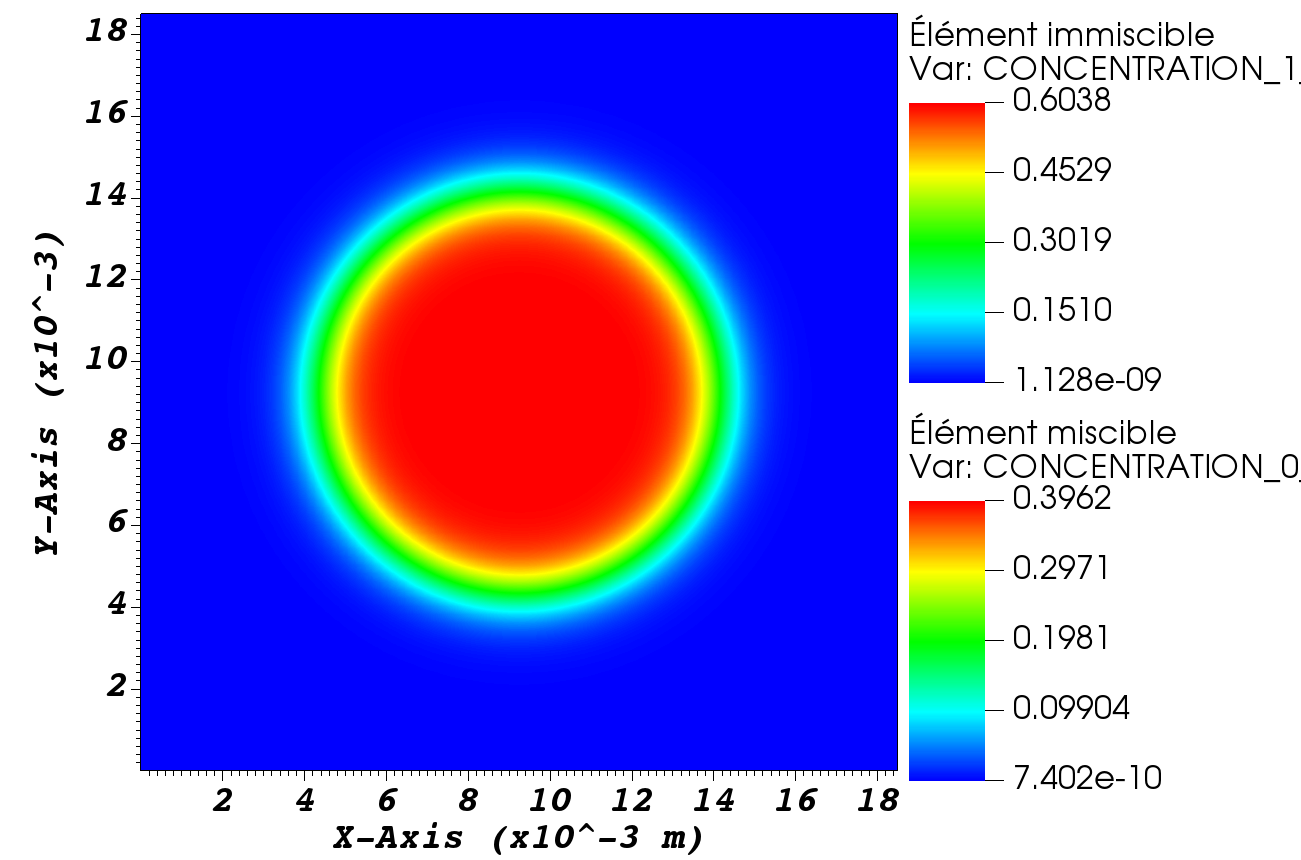
\includegraphics[width=0.5\linewidth]{figure/condition_init.png}
	\caption[Champ de concentration initiale]{Champ de concentration initiale, pour un domaine de taille $L_x = L_y = 18,5.10^{-3}$m des concentrations initiales de $\phi^{init,disp}_{misc} = 0,39,\phi^{init,disp}_{immi} = 0,60 $, un rayon de goutte de $R = 4,9.10^{-3}$m et une épaisseur d'interface $\epsilon = 8.10^{-4}$m }
	\label{fig:conditioninit}
\end{figure}

Contrairement au cas de présenté par Rao et al., nous faisons l'hypothèse d'une viscosité dynamique constante et commune pour l'ensemble des éléments du système. De plus la loi de densité linéaire proposée en équation \ref{eq:boussi} ne permet pas de garantir la conservation de l'ensemble des conditions initiales fournies par l'article \cite{rao_influence_2015}. En effet l'article fournit les masses volumiques des corps purs, de la goutte à l'état initial ainsi que les concentrations dans la goutte à l'état initial. Nous choisissons de conserver les masses volumiques des corps purs et de la goutte à l'état initial, modifiant ainsi sa composition initiale. Les coefficients de dilatation $\beta_{immi},\beta_{misc}$ sont déterminé à partir de la loi de densité \ref{eq:boussi} et des densités des corps purs :
\begin{subequations}
	\begin{empheq}[left={\empheqlbrace\,}]{align}
	&\rho(\phi^{misc} = 0, \phi^{immi} = 0) = \rho^* = \rho_{eau}\\
	&\rho(\phi^{misc} = 1, \phi^{immi} = 0) = \rho^*(1+ \beta_{misc}) = \rho_{misc}\\
	&\rho(\phi^{misc} = 0, \phi^{immi} = 1) = \rho^*(1+ \beta_{immi}) = \rho_{immi}
	\end{empheq}
\end{subequations}
avec $\rho_{eau},\rho_{misc},\rho_{immi}$ les masses volumiques des corps purs de l'eau, des composants miscible et immiscibles. Finalement les coefficients de dilatation s'écrivent : 
\begin{equation}
	\beta_{k} = \frac{\rho_{k}}{\rho_{eau}} - 1 
\end{equation}
avec $k = \{misc,immi\}$.
\section{Géométrie et maillage}
La \textit{baltik}\footnote{Dans TrioCFD, les \textit{baltiks} correspondent aux applications/solveurs} champ de phase (\textit{Phase-field}) se base sur une discrétisation VDF (Volume Différence Finies), cette discrétisation traite les vitesses sur les faces des mailles tandis que les champs scalaires (pression, température, paramètres d'ordre, masse volumique...) sont calculés au centre des mailles. De plus, tout au long de l'étude, nous utiliserons un maillage cartésien uniforme.
Il est également important de noter que le modèle étant encore en développement, il n'est pas possible de réaliser des calculs en parallèles. Les calculs étant longs, la convergence en maillage n'est pas assurée, l'effet de cette non-convergence est discuté au travers d'un exemple en section \ref{sec:raffinement}. De plus, pour des raisons de coût de calcul la taille du domaine utilisé ne peut pas être équivalente à celle de l'expérience proposée par Rao et al. et devient donc un paramètre de plus qui sera discuté en section \ref{sec:tailledom}. Les conditions aux limites de type symétrie étant également non-utilisable les calculs axisymétriques sont impossibles. L'ensemble des calculs sont donc réalisés en géométrie 2D cartésienne. L'épaisseur d'interface est supposée d'épaisseur égale à quatre mailles, l'impacte de cette épaisseur sur les résultats est discuté en section \ref{sec:raffinement}. Numériquement le choix a été fait de résoudre le terme diffusif de l'équation de Cahn-Hilliard en utilisant une méthode JFNK (\textit{Jacobian-Free Newton-Krylov}) associé à un solveur GMRES (\textit{Generalized Minimal RESidual}), le terme d'advection ainsi que les équations de l'hydrodynamique sont résolus avec une méthode de Range-Kutta d'ordre 3. Le pas de temps est supposé constant est égale à $dt = 10^{-4}$s pour l'ensemble des simulations. Un schéma représentatif du domaine et du maillage est présenté en Figure \ref{fig:Presentation_Dom}.
%Finalement au cours de ce travail on cherche à démontrer la capacité du code à réaliser une simulation couplant hydrodynamique et transfert de masse sans proposer une validation complète.

\begin{figure}[H]
	\centering
	\small
	\begin{tikzpicture}
	\filldraw[color=red!60, fill=red!5, very thick](0,-1) circle (0.8);
	\draw[step=0.5cm,gray,very thin] (-2,-2) grid (2,6);
	\draw[>=triangle 45, <->,very thin] (-2,-2.3) -- (2,-2.3);
	\draw[>=triangle 45, <->] (2.3,-2) -- (2.3,6);
	\node[] at (0,-2.6) {$L_x$};
	\node[] at (2.6,2) {$L_y$};
	\draw [to-to] (-2.1,6) -- (-2.1,5.55);
	\node[] at (-2.4,5.8) {$dy$};
	\draw [to-to] (-2,6.1) -- (-1.55,6.1);
	\node[] at (-1.8,6.3) {$dx$};
	\draw [to-to] (0,-1) -- (0.7,-1.2);
	\node[] at (0.9,-1.2) {$R$};
	\node[] at (-0.,-0.7) {$(x_0,y_0)$};
	\end{tikzpicture}
	\caption{Schéma du domaine de calcul et des conditions aux limites}
	\label{fig:Presentation_Dom}
\end{figure}

\section{Paramétrage du paysage thermodynamique}
\subsection{Critères d'admissibilité} \label{subsec:critere_admi}
Dans cette section, les critères de choix du paysage thermodynamique seront présentés. En effet, contrairement au cas du corium, il n'existe pas de base thermodynamique pour le système acétonitrile/chlorobenzène. Ce manque d'information thermodynamique force à choisir arbitrairement un paysage et ne permet pas de mener une étude de validation quantitative. Cependant certains critères de choix existent et permettent de savoir si un paysage est potentiellement cohérent avec le système étudié.
Dans un premier temps, il est essentiel que les conditions initiales ne soient pas incluses dans la lacune de miscibilité, ce qui entraînerait une séparation de phase immédiate. Un exemple de paysage est donné en Figure \ref{fig:landscapebase} et les résultats sont présentés en Figure \ref{land_base_sep}. On y observe une séparation de phase dès les premiers instants du calcul avec la présence de deux phases à l'intérieur de la goutte, une première uniquement composée de l'élément immiscible et la seconde composée d'eau et de l'élément miscible.
 \begin{figure}[H]
 	\centering
 	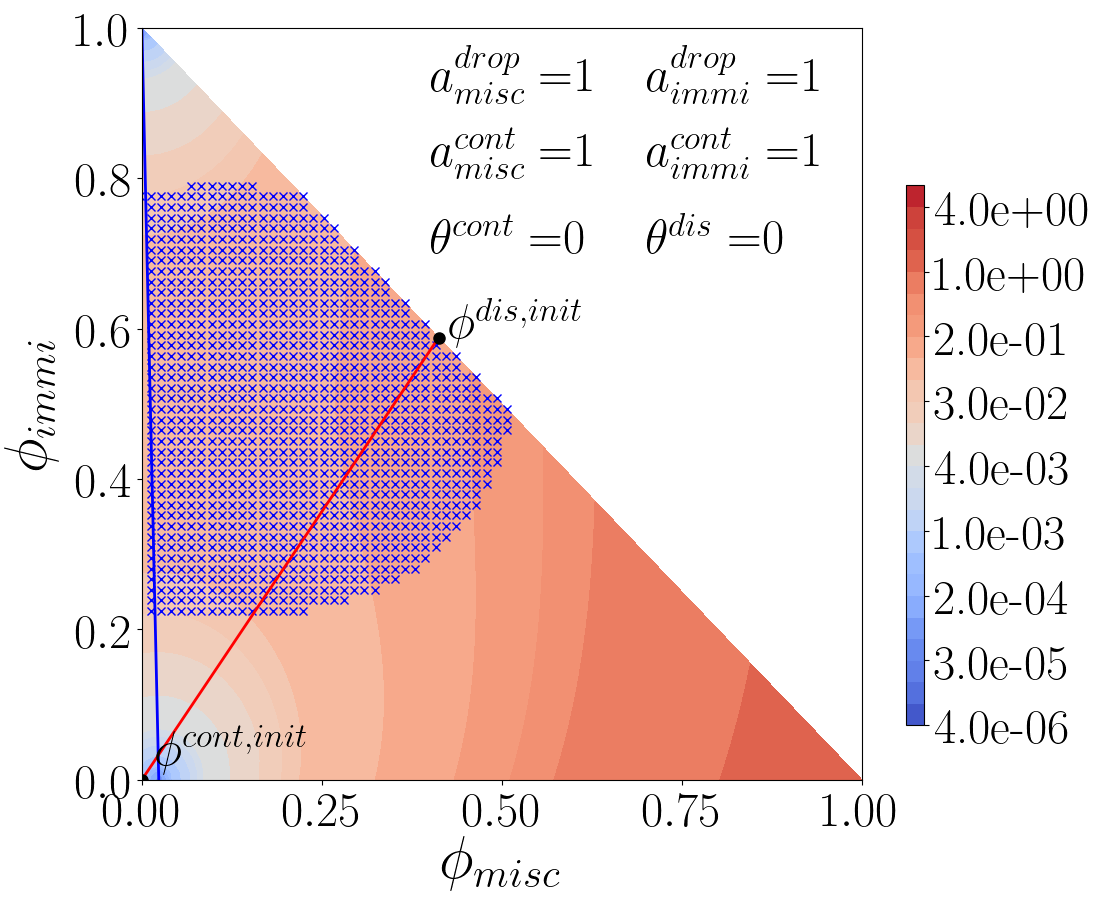
\includegraphics[width=0.6\linewidth]{figure/landscape_base_chap3.png}
 	\caption[Paysage thermodynamique]{Paysage thermodynamique, la droite bleu relie les deux concentrations d'équilibre, la droite rouge relie les deux concentrations initiales}
 	\label{fig:landscapebase}
 \end{figure}
\vspace{-0.5cm}
% \begin{figure}[H]
% 	\centering
% 	\begin{subfigure}[H]{0.32\textwidth}
% 		\centering
% 		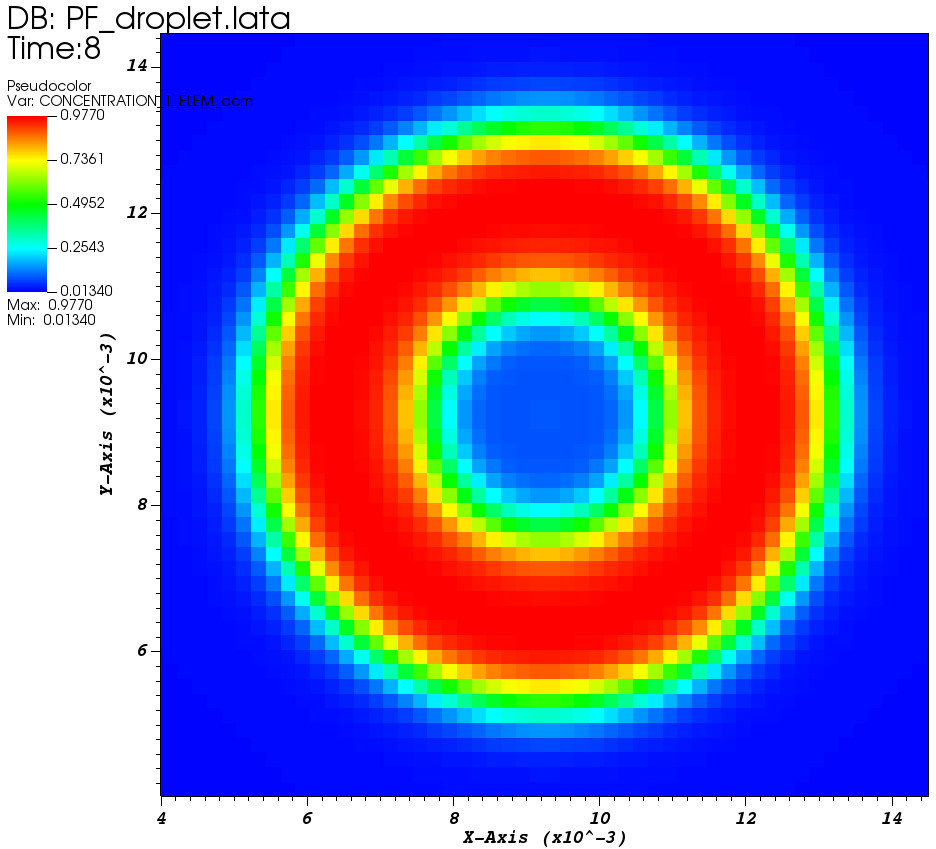
\includegraphics[width=\textwidth]{figure/paysage_base/visit0000.png}
% 		\caption{Concentration de l'élément immiscible}
% 		\label{fig:y equals x}
% 	\end{subfigure}
% 	\begin{subfigure}[H]{0.32\textwidth}
% 		\centering
% 		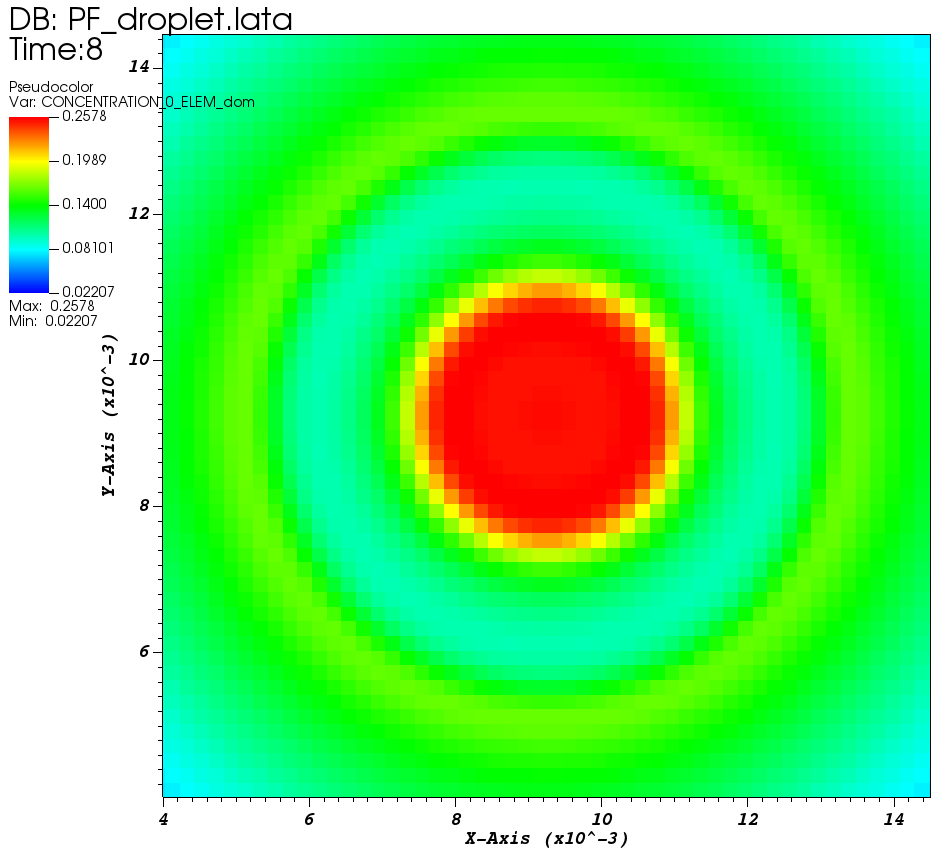
\includegraphics[width=\textwidth]{figure/paysage_base/visit0001.png}
% 		\caption{Concentration de l'élément miscible}
% 		\label{fig:y equals x}
% 	\end{subfigure}
% 	\begin{subfigure}[H]{0.32\textwidth}
% 		\centering
% 		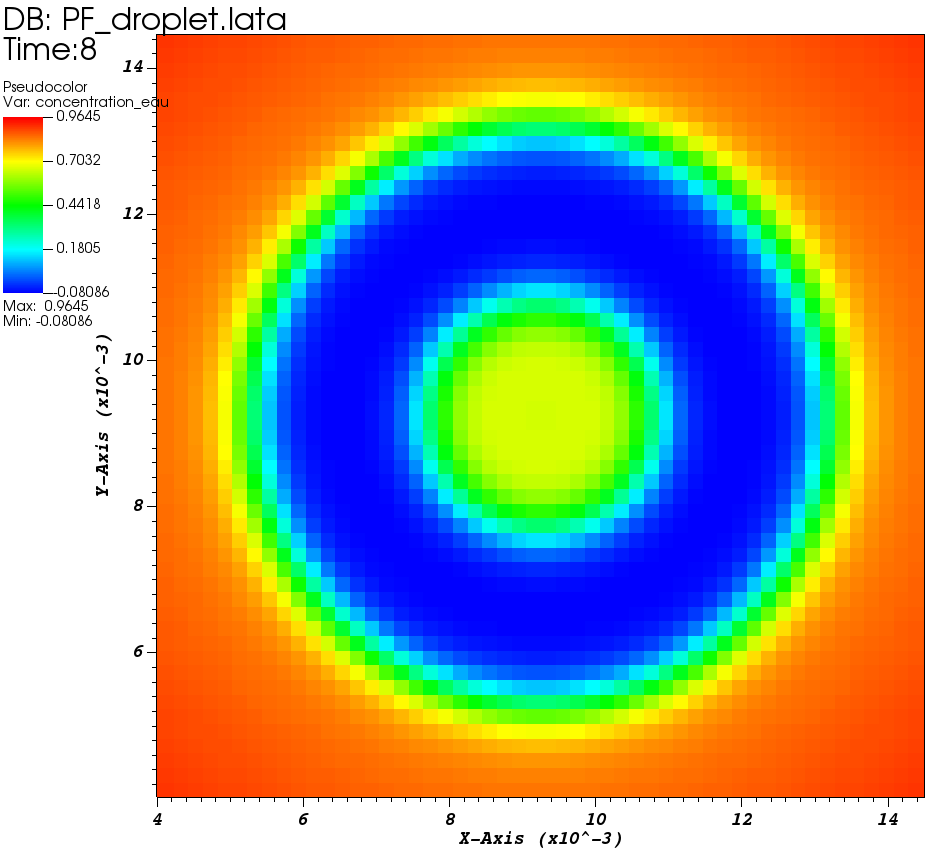
\includegraphics[width=\textwidth]{figure/paysage_base/visit0002.png}
% 		\caption{Concentration d'eau}
% 		\label{fig:y equals x}
% 	\end{subfigure}
% 	\caption{Séparation de phase dans la goutte}
% 	\label{land_base_sep}
% \end{figure} \vspace{-0.5cm}
 \begin{figure}[H]
	\centering
	\begin{subfigure}[H]{0.4\textwidth}
		\centering
		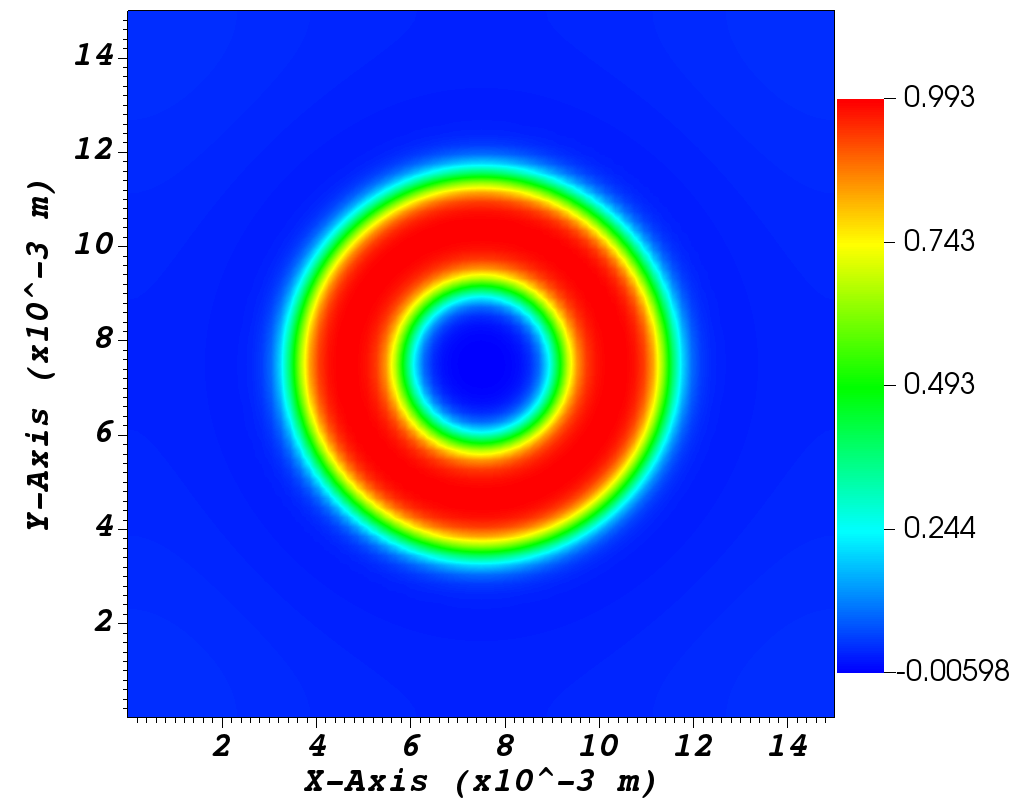
\includegraphics[width=1\textwidth]{figure/separation_immi.png}
		\caption{Concentration de l'élément immiscible}
		\label{fig:y equals x}
	\end{subfigure} \hfil
	\begin{subfigure}[H]{0.4\textwidth}
		\centering
		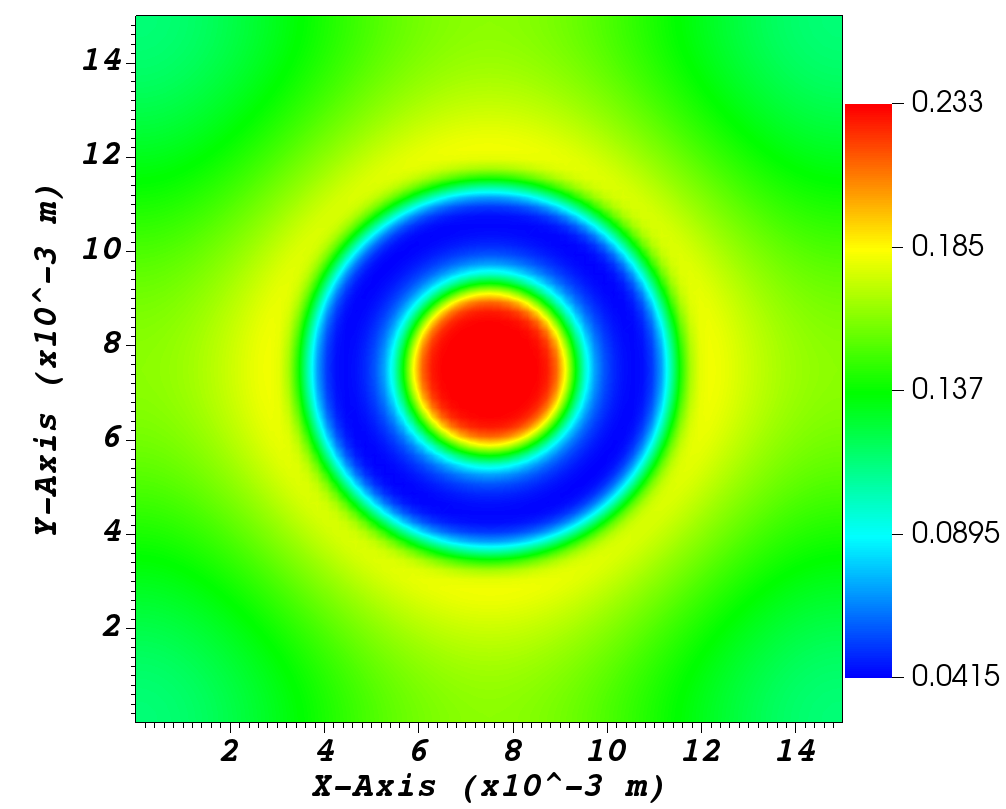
\includegraphics[width=1\textwidth]{figure/separation_misc.png}
		\caption{Concentration de l'élément miscible}
		\label{fig:y equals x}
	\end{subfigure}
	\caption{Séparation de phases dans la goutte à $t=9s$, pour un domaine de taille $L_x = L_y = 15.10^{-3}$m des concentrations initiales de $\phi^{init,disp}_{misc} = 0,39,\phi^{init,disp}_{immi} = 0,60 $, un rayon de goutte de $R = 4,9.10^{-3}$m et une épaisseur d'interface $\epsilon = 8.10^{-4}$m, une mobilité de $\mathcal{M} = 10^{9}$m$^2$.s$^{-1}$ en utilisant le paysage présenté en Figure \ref{fig:landscapebase}}
	\label{land_base_sep}
\end{figure} \vspace{-0.5cm}
Le deuxième critère est associé à l'évolution initiale du système, un deuxième paysage est présenté en Figure \ref{fig:paysage_thermo_grad}. En effet, l'objectif est également de limiter l'entrée d'eau dans la goutte, pour cela il est nécessaire qu'en tout point de la goutte la somme des compositions des composants miscible et immiscible soit égale à l'unité. Pour que cela soit toujours le cas, il est important que l'orientation des gradients soit favorable dès l'instant initial. La Figure \ref{fig:gradpasbon} présente un exemple où ce gradient favorise une entrée d'eau dès les premiers instants, dans cet exemple le gradient favorise également un chemin qui passe par la zone instable. Ainsi, il est également possible de prévoir une séparation de phase, l'ensemble de ces phénomènes peuvent être observés sur la Figure \ref{fig:eauref}, l'entrée d'eau est visible dès les premiers instants (t$=0.3$s), la séparation de phase apparaît sur des temps intermédiaires (t$=10$s et t$=25$s) pour finalement retrouver l'état stationnaire attendu d'une goutte homogène ne contenant pas d'eau pour des temps longs (t$=50s$).

%Comme expliqué précédemment ce paysage représente l'énergie libre volumique liée à l'équilibre des phases, ainsi on cherche à ce que les conditions initiales (ici aux extrémités de la droite rouge) soit hors de la zone instable et que la composition d'équilibre globale (placé a l'intersection des droites bleu et rouge) soit placée dans la lacune de miscibilité. Ainsi ce paysage semble correspondre parfaitement à ces deux critères. On souhaite également limiter l'entrée d'eau dans la goutte en régime transitoire, cette condition ce traduit par égalité entre la somme des deux compositions et l'unité. Hors ici le gradient d'énergie favorise un "chemin" différent. Pour vérifier cette présence d'eau, on considère alors un calcul statique (sans résolution des équations de Navier-Stokes) et on trace les concentrations à différents instants. On observe dès lors une importante intrusion d'eau dans la goutte dès les premiers instants, puis une séparation de phase est observable à l'intérieur de la goutte, phénomène que l'on souhaite absolument éviter.
 \begin{figure}[H]
 	\centering
 	\begin{subfigure}[H]{0.45\textwidth}
 		\centering
 		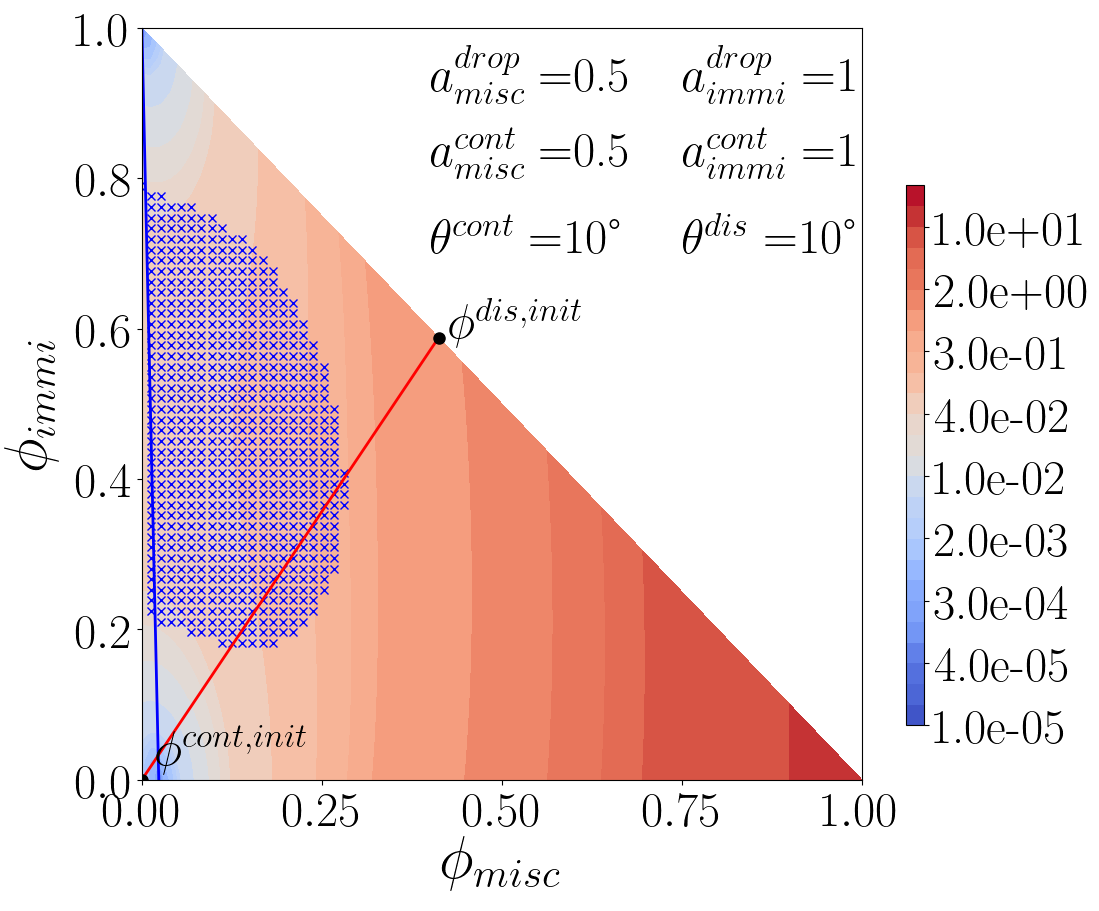
\includegraphics[width=1.2\textwidth]{figure/paysage_neqlocal}
 		\caption{Paysage thermodynamique complet}
 		\label{fig:paysage_thermo_grad}
 	\end{subfigure}
 	\hfill
 	\begin{subfigure}[H]{0.45\textwidth}
 		\centering
 		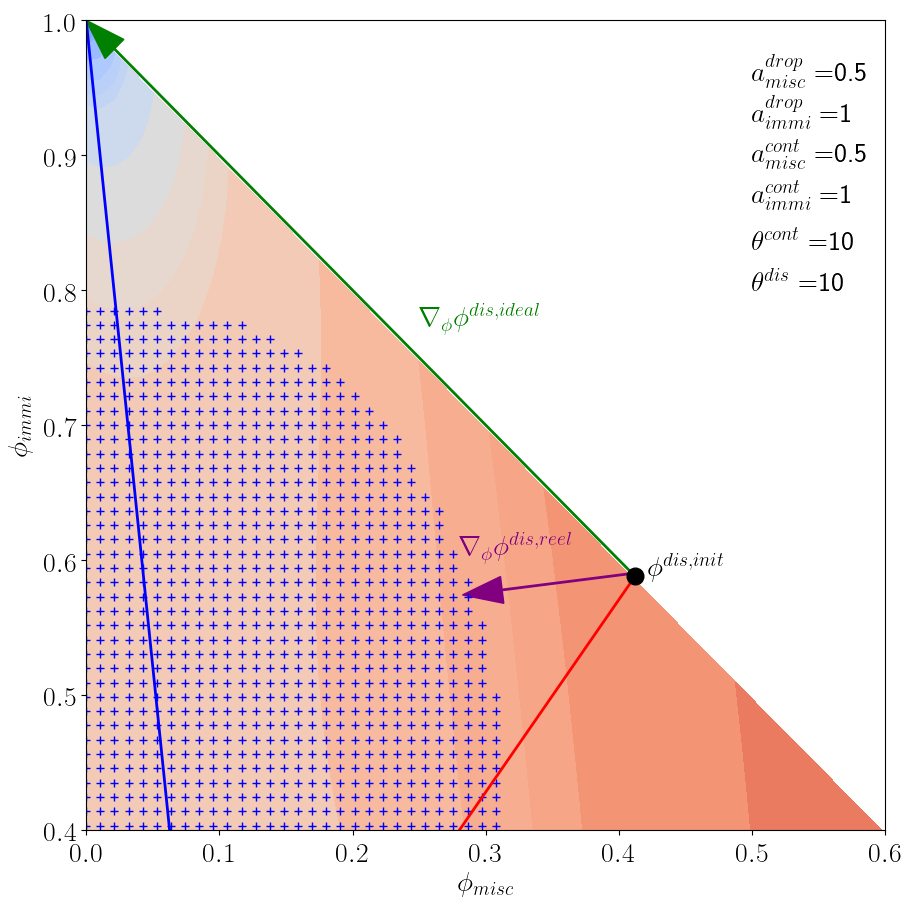
\includegraphics[width=\textwidth]{figure/direction_gradient}
 		\caption{Paysage thermodynamique partiel}
 		\label{fig:gradpasbon}
 	\end{subfigure}
 	\caption{Paysage thermodynamique et direction privilégiée par le système, la flèche verte représente le cas idéal sans intrusion d'eau et la flèche violette le cas associé au paysage thermodynamique, la zone bleu correspond à la zone instable}
 	\label{fig:paysage_thermo_gradglob}
 \end{figure}\vspace{-0.7cm}
 \begin{figure}[H]
 	\centering
 	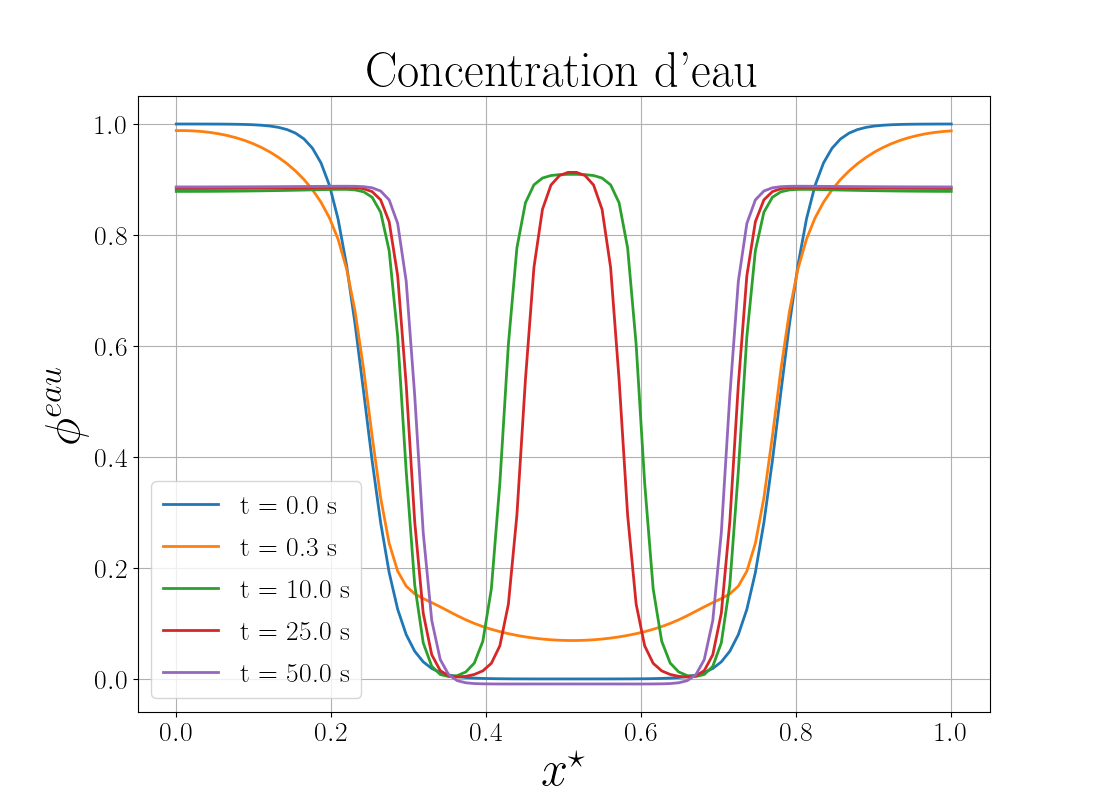
\includegraphics[width=0.5\linewidth]{figure/eau_ref}
 	\caption[Concentration d'eau dans le domaine]{Profil de la concentration d'eau dans le domaine, $x^{\star} = x / L_x$ représente une longueur adimensionnée}
 	\label{fig:eauref}
 \end{figure}\vspace{-0.7cm}
Finalement, au travers de ces deux exemples, nous avons illustré les pathologies auxquelles un choix inadapté de paysage thermodynamique peut conduire. Les critères concernent la position des conditions initiales, qui doivent être en dehors de la zone instable, un second critère concerne l'absence nécessaire de la zone instable sur le "chemin" de chacune des phases et finalement une direction initiale privilégiant l'absence d'eau dans la goutte.
\subsection{Choix d'un paysage et simulations sans couplage avec l'hydrodynamique}
Éviter les pathologies précédentes s'avère très contraignant dans le choix des paramètres du potentiel analytique. Divers tests ont mené au passage présenté à la Figure \ref{fig:thechoosenone} pour lequel nous allons maintenant analyser plus en détails le comportement de la goutte.
\begin{figure}[H]
		\centering
		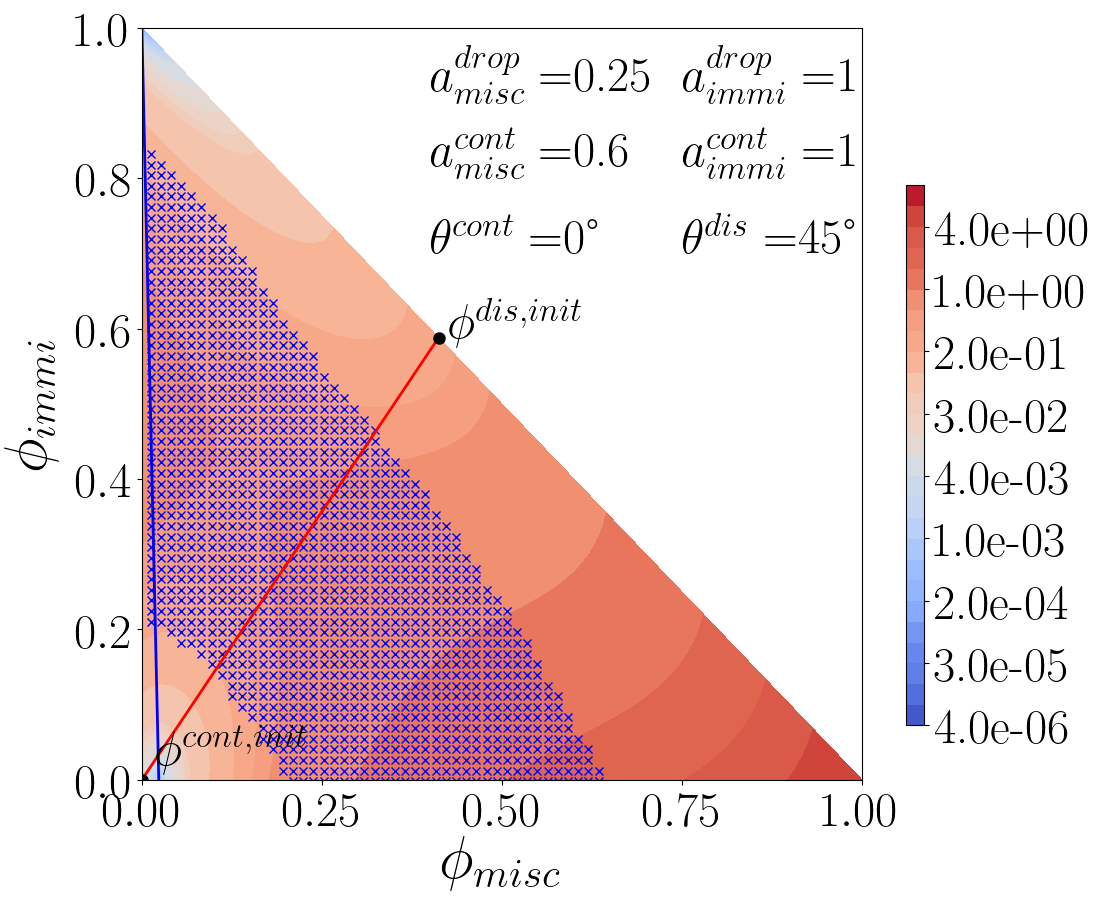
\includegraphics[width=0.6\textwidth]{figure/Paysage_ecriture1.png}
	\caption{Paysage thermodynamique choisit pour la simulation}
	\label{fig:thechoosenone}
\end{figure}

Pour démontrer la consistance de ce paysage, une simulation sans couplage avec les équations de Navier-Stokes est réalisée. La Figure \ref{fig:resultstatiquegoodlandscape} présente les résultats, il est possible d'observer que ce paysage préserve la goutte des pathologies présentées en section \ref{subsec:critere_admi}. En effet, on n'observe pas de séparation de phases ni d'intrusion d'eau. Les profils de concentration sur des temps courts (t<5s) ne présentent pas d'anomalie, cependant sur des temps plus long une non-monotonie de l'interface pour le composant miscible est observée. De plus à l'intérieur de la goutte, la concentration de composant miscible est négative et la composition d'élément immiscible est quant à elle supérieure à 1, tel que la somme des deux concentrations soit égale à l'unité. Certaines solutions existent pour limiter l'apparition de valeurs incohérente de concentration (i.e. $\phi_{i}^k \notin [0,1]$), une des solutions est d'utiliser une mobilité dégénérée, ainsi la mobilité devient fonction des paramètres d'ordre. La non monotonie, quant à elle, est liée à une adsorption d'interface, une étude plus complète est présente en annexe \ref{absorption}. Finalement, ces problèmes sont principalement présents pour des temps supérieurs aux temps d'intérêt de nos simulations, nous faisons donc l'hypothèse que ce paysage peut, malgré ses défauts et dans un premier temps, convenir pour nos simulations. Une étude des profils de concentration lors d'une simulation couplée est présentée en section \ref{sec:calibmo}.
\begin{figure}[H]
	\centering \hspace{-2cm}
	\begin{subfigure}[H]{0.45\textwidth}
		\centering
		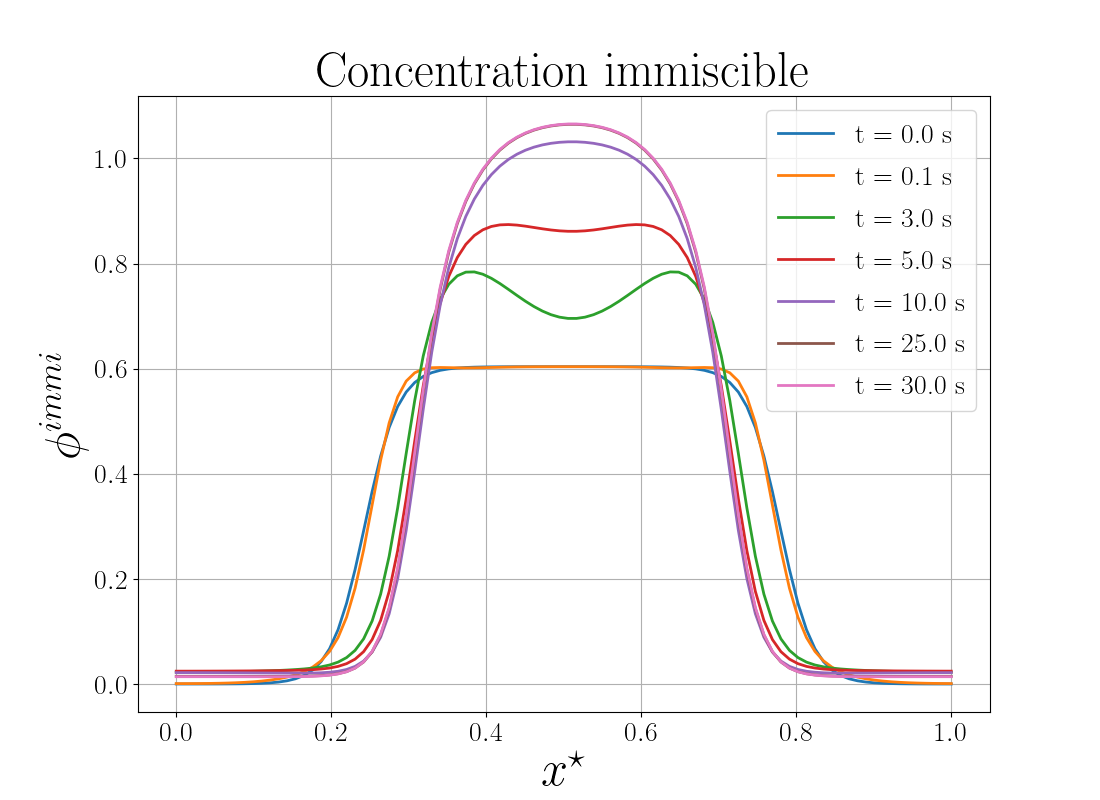
\includegraphics[width=1.1\textwidth]{figure/nouveau_parametrage/immiscible_New_Parametrage.png}
		\caption{Concentration immiscible}
		\label{fig:y equals x}
	\end{subfigure} \hfil
	\begin{subfigure}[H]{0.45\textwidth}
		\centering
		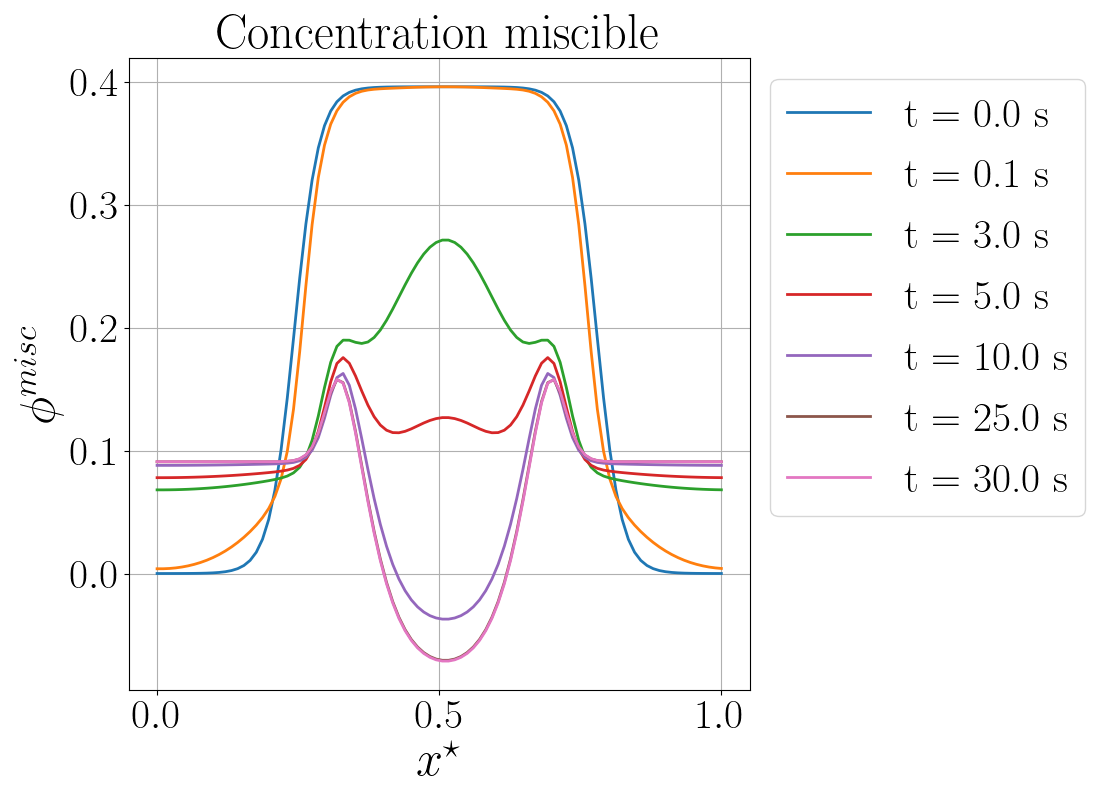
\includegraphics[width=1.1\textwidth]{figure/nouveau_parametrage/miscible_New_Parametrage.png}
		\caption{Concentration miscible}
		\label{fig:y equals x}
	\end{subfigure}
\end{figure} \vspace{-0.8cm}
\begin{figure}[H]
	\centering
	\ContinuedFloat
	\begin{subfigure}[H]{0.45\textwidth}
		\centering
		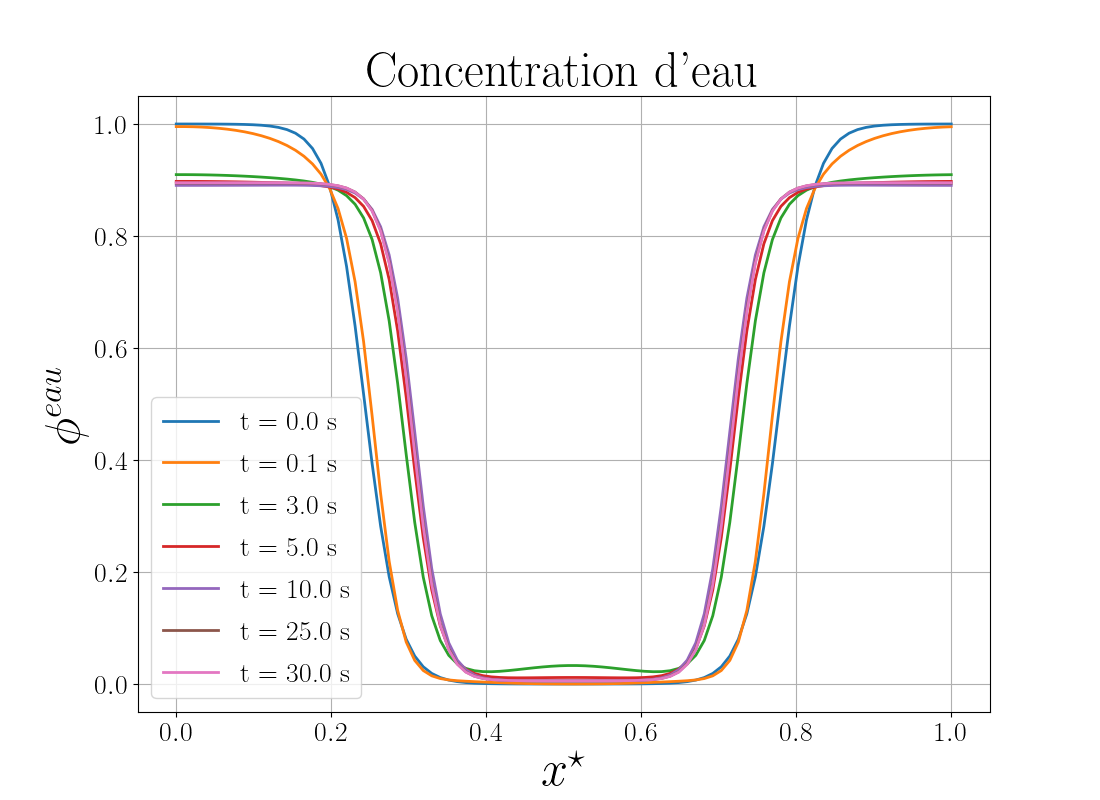
\includegraphics[width=1.1\textwidth]{figure/nouveau_parametrage/eau_New_Parametrage.png}
		\caption{Concentration d'eau}
	\end{subfigure}
	\caption{Variation de la concentration des différents composants au cours du temps}
	\label{fig:resultstatiquegoodlandscape}
\end{figure}
%\subsection{Effet de la courbure sur le profil d'interface}
%
%Au vu des résultats précédent il est possible de ce demander si le profil non monotone de l'interface n'est pas dû à la courbure de l'interface (effet de Gibbs-Thomson). En effet aucune solution analytique ne tient compte d'une courbure. Ainsi on compare deux systèmes parfaitement identique à l'exception de la courbure de l'interface. Un premier système possède une interface plane et le second une interface courbée. On présente les résultats en figure \ref{fig:planemiscible}. \vspace{-0.1cm}
%\begin{figure}[H]
%	\centering
%	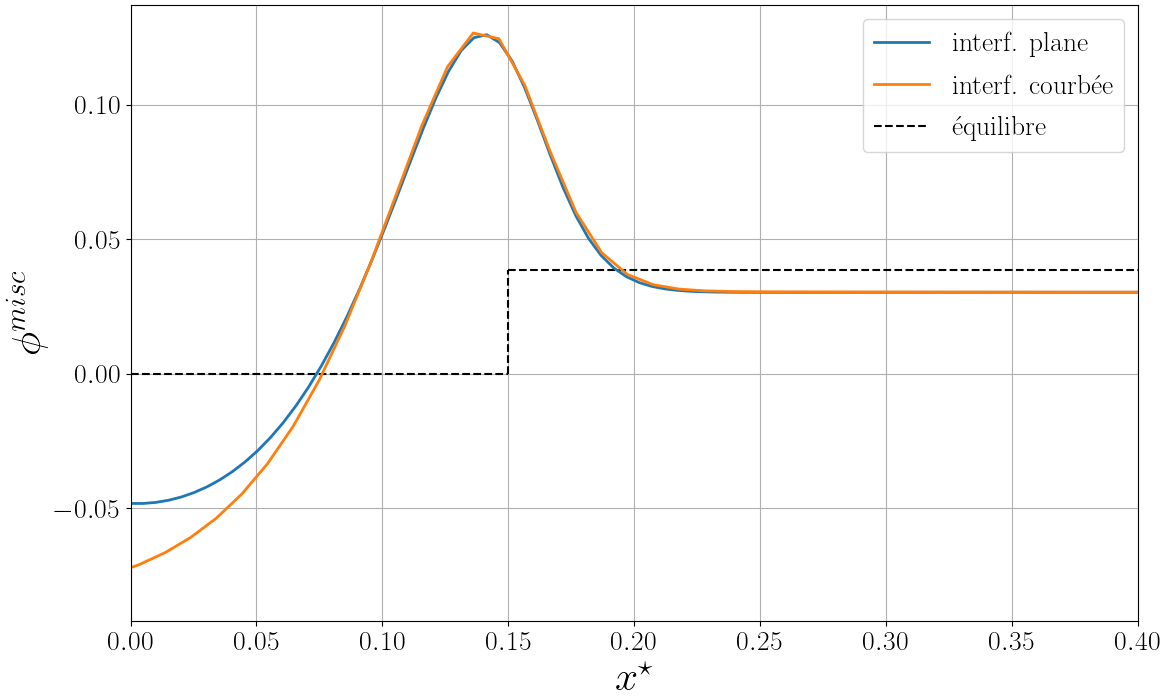
\includegraphics[width=0.5\linewidth]{figure/plane_miscible}
%	\caption[Profils de concentration du composant miscible pour une interface plane ou courbée]{Profils de concentration du composant miscible pour une interface plane ou courbée}
%	\label{fig:planemiscible}
%\end{figure}
%On y observe que la courbure de l'interface influe uniquement sur la valeur à l'équilibre dans la goutte mais pas sur le profil d'interface. Finalement cette non monotonie ne semble pas en lien avec avec la courbure.
\section{Simulations couplées et comparaison à l'expérience}

Malgré la non-monotonie de l'interface, le couplage avec l'hydrodynamique est envisageable. En effet, la non-monotonie semble apparaître pour des temps longs, supérieurs aux temps que l'on souhaite observer dans notre étude. Ainsi, pour la suite de ce travail on considère des simulations couplées Cahn-Hilliard/Navier Stokes.
\subsection{Calibration de la mobilité et étude du comportement de la goutte} \label{sec:calibmo}
La mobilité est un paramètre cinétique qui modélise la compétition entre la diffusion massique et l'hydrodynamique. Le transfert de masse étant principalement piloté par le paysage thermodynamique, la valeur de la mobilité se doit d'être en accord avec ce dernier. Dans le cas présent, le paysage est analytique et les ordres de grandeurs physiques ne sont pas respectés. C'est pourquoi la mobilité est utilisée comme paramètre de calage. Les paramètres relatifs aux simulations sont présentés en Table \ref{table:cas_ref}.
\begin{table}[H]
	\centering  % not needed, since table is as wide as text block
	\begin{tabularx}{\textwidth}{@{}lYYYYYY@{}}
		\toprule
		&\multicolumn{6}{c}{\bfseries Géométrie et maillage}\\
		%\cmidrule(lr){2-3} \cmidrule(l){4-5} 
		& $L_x$ (m)
		& $L_y$ (m)
		& $dx, dy$ (m)
		& $N_x$
		& $N_y$
		& $D^{drop}$  (m)\\
		\midrule
		Valeurs  & 2,45.10$^{-2}$ & 15.10$^{-2}$ & 2.10$^{-4}$ & 123 & 750 & 4,9.10$^{-3}$ \\
		\bottomrule
	\end{tabularx}
\end{table} \vspace{-0.8cm}
\begin{table}[H]
	\begin{tabularx}{\textwidth}{@{}lYYYYYY@{}}
		\toprule
		&\multicolumn{6}{c}{\bfseries Paramètres physiques}\\
		%\cmidrule(lr){2-3} \cmidrule(l){4-5} 
		& $\rho^*$ (kg.m$^{-3}$)
		& $\eta$ (Pa.s)
		& $\beta_{misc}$ (-)
		& $\beta_{immi}$ (-)
		& $\epsilon$ (m)
		& $\sigma$ (N.m$^{-1}$)\\
		\midrule
		Valeurs & 999,5 & 10$^{-3}$& -0,21 & 0,10 & 8.10$^{-4}$ & 36.10$^{-3}$ \\
		\bottomrule
	\end{tabularx}
\end{table}\vspace{-0.8cm}
\begin{table}[H]
	\begin{tabularx}{\textwidth}{@{}lYYYY@{}}
		\toprule
		&\multicolumn{3}{c}{\bfseries Paramètres "champ de phase"}\\
		%\cmidrule(lr){2-3} \cmidrule(l){4-5} 
		& $\lambda$ (-)
		& $\kappa$
		& $\mathcal{M}$ (m$^2$.s$^{-1}$)\\
		\midrule
		Valeurs  & 22,87 & 4,32.10$^{-5}$ $\delta_{ij}$ & \{\textcolor{blue}{5.10$^{-8}$},\textcolor{orange}{1.10$^{-8}$}, \textcolor{green}{5.10$^{-9}$}, \textcolor{red}{4.10$^{-9}$}, \textcolor{purple}{1.10$^{-9}$}, \textcolor{brown}{1.10$^{-12}$}\} $\delta_{ij}$ \\	
		\bottomrule
	\end{tabularx}
\end{table}\vspace{-0.8cm}
\begin{table}[H]
	\begin{tabularx}{\textwidth}{@{}lYYYYYYYY@{}}
		\toprule
		&\multicolumn{8}{c}{\bfseries Conditions initiales et d'équilibres}\\
		%\cmidrule(lr){2-3} \cmidrule(l){4-5} 
		& $\phi_{misc}^{drop}$ 
		& $\phi_{immi}^{drop}$ 
		& $\phi_{misc}^{cont}$ 
		& $\phi_{immi}^{cont}$
		& $\phi_{misc}^{drop,eq}$ 
		& $\phi_{immi}^{drop,eq}$ 
		& $\phi_{misc}^{cont,eq}$ 
		& $\phi_{immi}^{cont,eq}$ \\
		\midrule
		Valeurs  & 0,42 & 0,58 & 0 & 0 & 0 & 1 & 2.10$^{-3}$ & 0\\
		\bottomrule
	\end{tabularx}
	\caption{Paramètres de simulation} \label{table:cas_ref}
\end{table}
\noindent La position de la goutte $y_G(t)$ à l'instant $t$ est obtenue tel que :
\begin{equation}
		y_G(t) = \cfrac{\int_V y \times \phi_{immi}(t,\mathbf{x}) dV }{\int_V  \phi_{immi}(t,\mathbf{x}) dV}
\end{equation}
Ainsi pour déterminer la valeur de la mobilité, les trajectoires obtenues pour différentes mobilités sont comparées avec la trajectoire de référence fournie par Rao et al. en figure \ref{fig:trajectoireexp4}.
\begin{figure}[H]
	\centering
	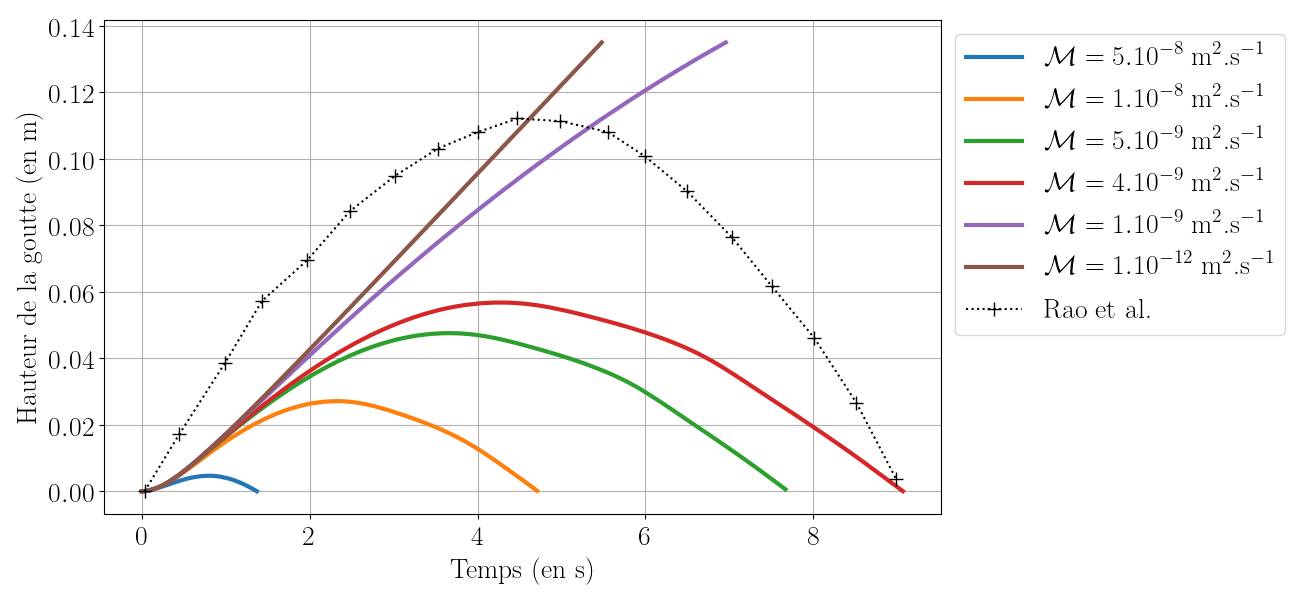
\includegraphics[width=0.9\linewidth]{figure/trajectoire_Exp4}
	\caption[Trajectoire de la goutte]{Trajectoire de la goutte pour différentes mobilités}
	\label{fig:trajectoireexp4}
\end{figure}
Il est possible d'observer qu'aucune trajectoire ne semble correspondre, en termes d'amplitude, avec celle de l'expérience. Cette différence est certainement la cause d'une mauvaise estimation de la loi de densité. Cependant, il est possible de remarquer qu'une mobilité de l'ordre de $\mathcal{M} = 4.10^{-9}$ m$^2$.s$^{-1}$ permet d'obtenir des instants d'inversion de densité cohérents. C'est pourquoi pour la suite de ce travail une mobilité égale à cette valeur est considérée. Pour vérifier l'impact mineur de la non-monotonie de l'interface caractérisé précédemment, nous traçons les profils de concentration dans la goutte pour différents instants dans le cas d'une simulation couplée avec la mobilité de référence choisie. Ces profils de concentrations sont présentés en Figure \ref{fig:verifcouplage}. On y observe bien l'apparition de la non-monotonie aux temps longs de la simulation (t>6s). Pour nos temps de simulation, l'amplitude de la non-monotonie reste très faible et nous supposons l'effet négligeable, nous confortant ainsi dans l'utilisation du paysage choisi. Nous pouvons également observer, que les résultats sont identiques pour la première seconde de calcul (à l'exception d'une mobilité très forte $\mathcal{M} = 5.10^{-8}$m$^2$.s$^{-1}$). Ainsi, on en déduit que l'hydrodynamique domine aux temps courts.
\begin{figure}[H]
	\centering
	\begin{subfigure}[H]{0.45\textwidth}
		\centering
		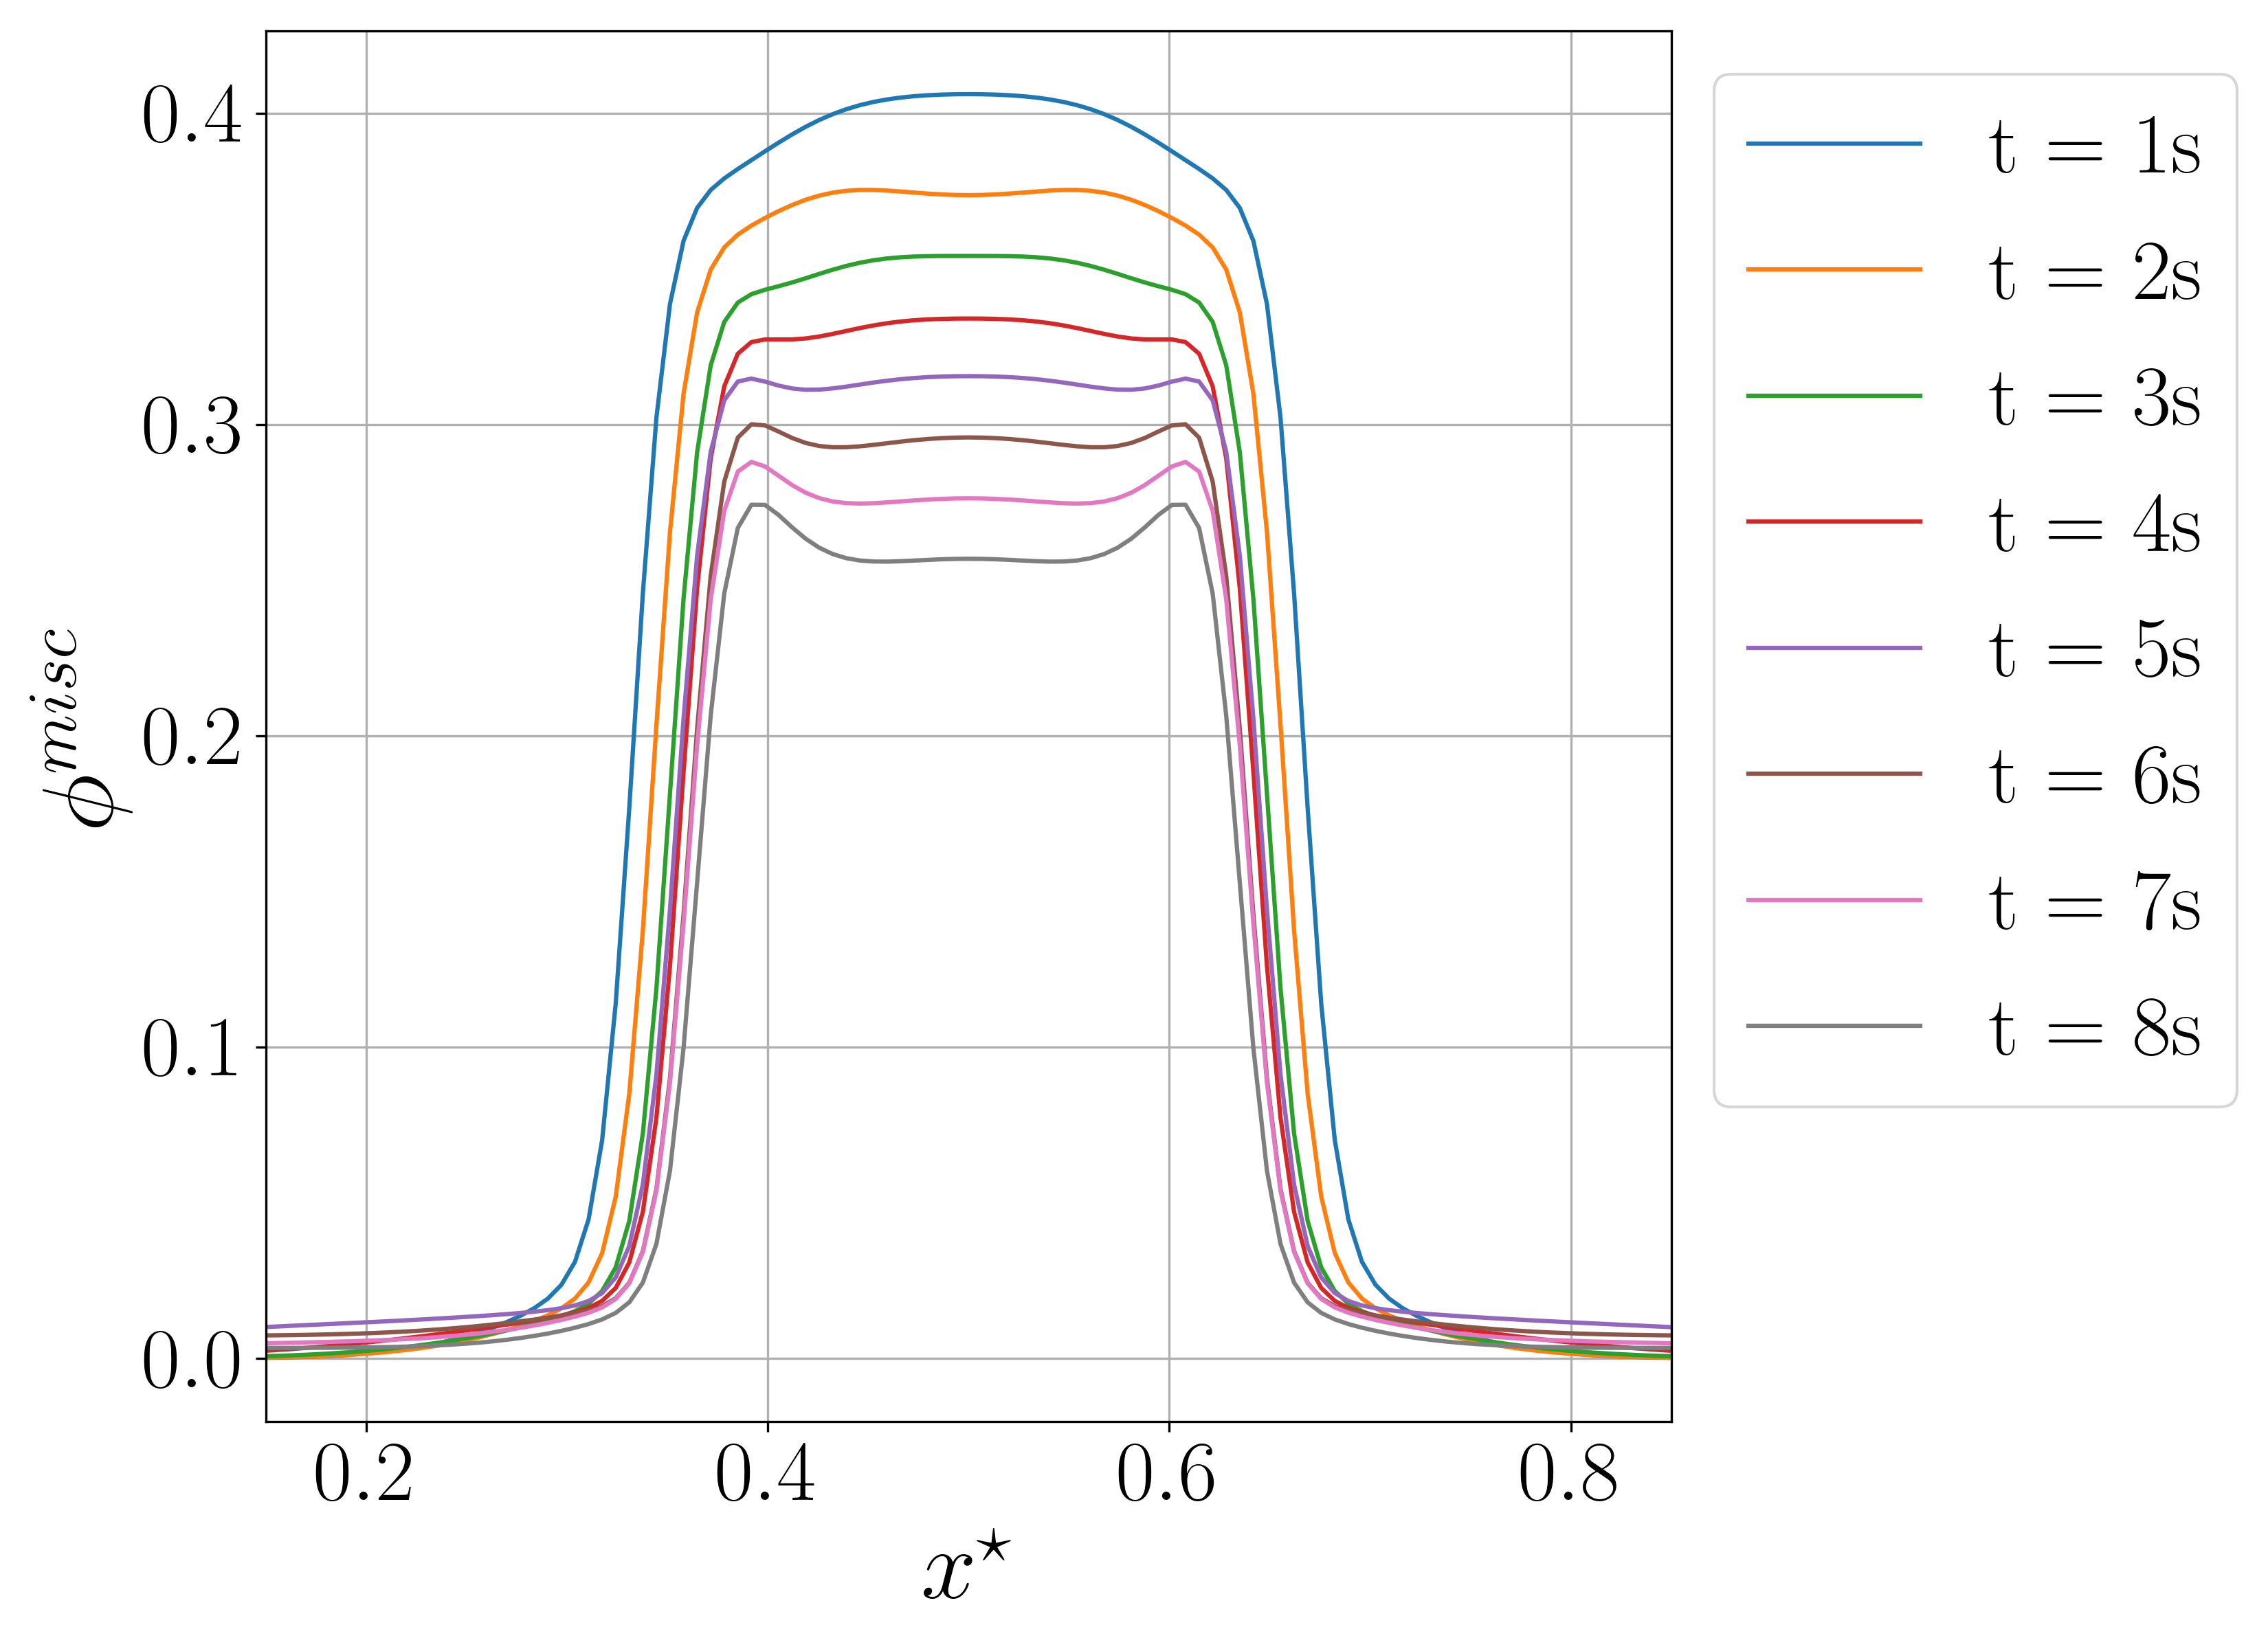
\includegraphics[width=1.1\textwidth]{figure/miscible_NS.png}
		\caption{Élément miscible}
		\label{fig:y equals x}
	\end{subfigure} \hfill
	\begin{subfigure}[H]{0.45\textwidth}
		\centering
		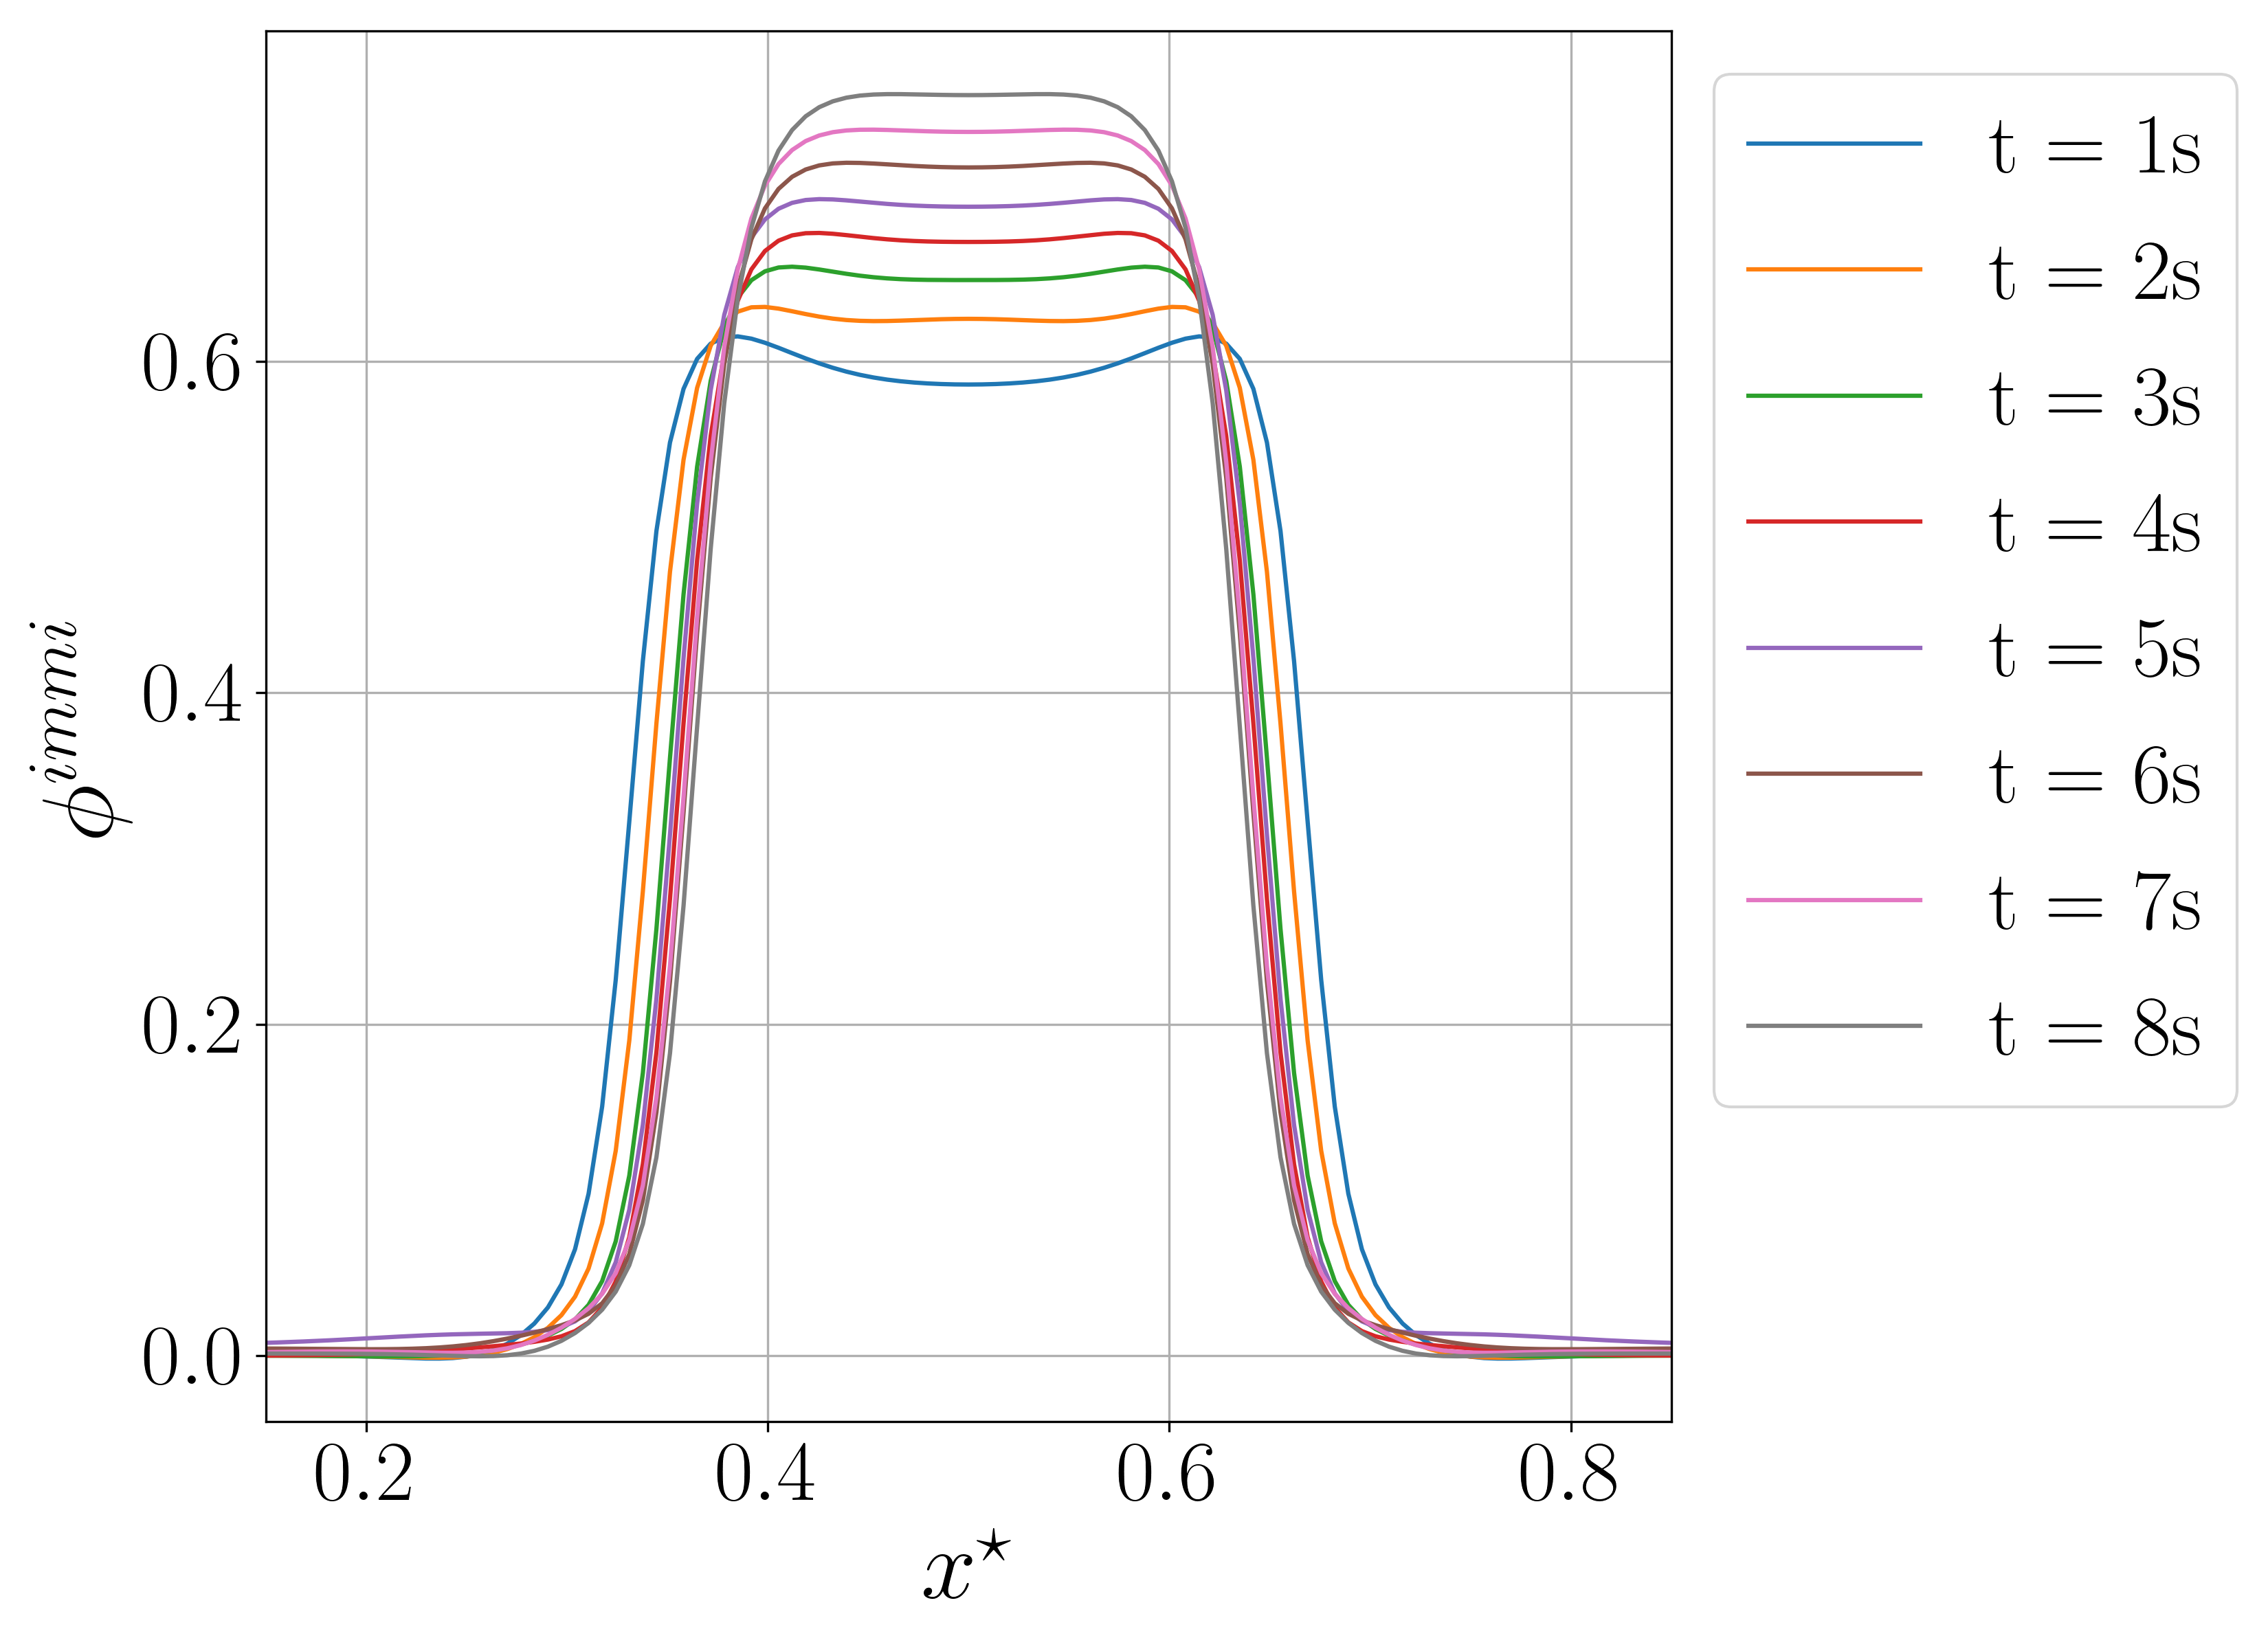
\includegraphics[width=1.1\textwidth]{figure/immiscible_NS.png}
		\caption{Élément immiscible}
		\label{fig:y equals x}
	\end{subfigure}
	\caption{Profil de concentration des éléments miscible et immiscible dans la goutte pour un simulation couplée CH/NS}
	\label{fig:verifcouplage}
\end{figure}




L'article de Rao et al. présente également des résultats sur la vitesse de la goutte. La vitesse est obtenue en dérivant la position de la goutte telle que formulé par l'équation \ref{eq:vitessegoutte}. Les résultats de vitesse de goutte sont présentés en Figure \ref{fig:vitesseexp4}.
	\begin{equation} \label{eq:vitessegoutte}
	u_y^{n+1} = \cfrac{y_G^{n+1} - y_G^{n}}{t^{n+1}- t^n}
\end{equation}
\begin{figure}[H]
	\centering
	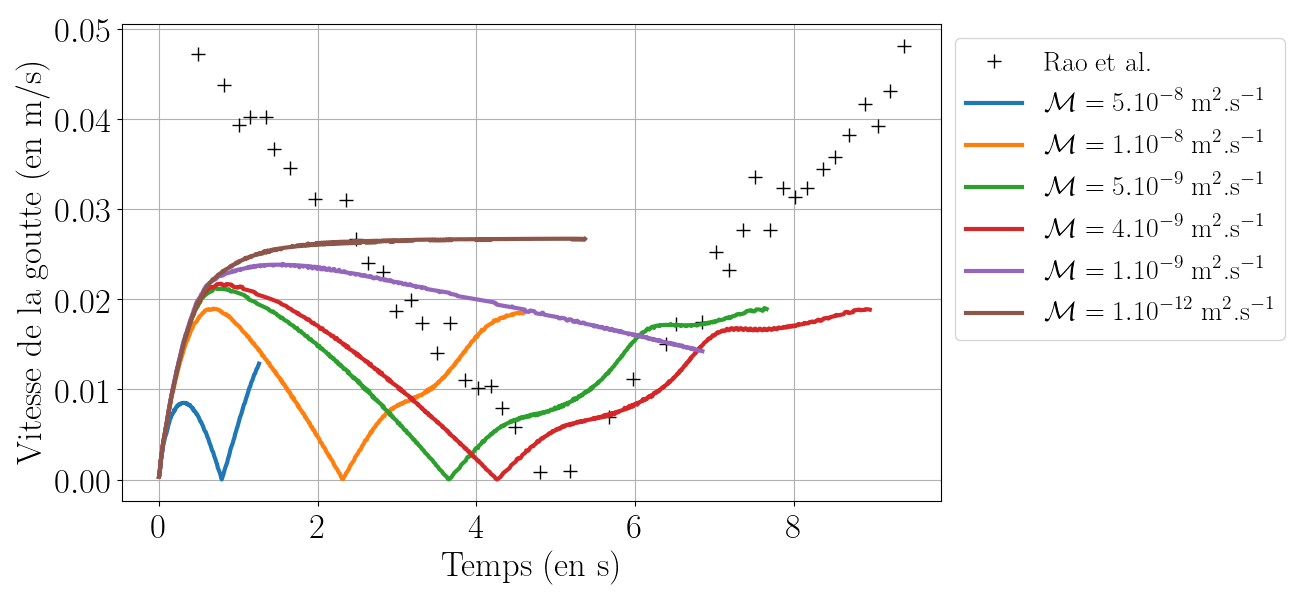
\includegraphics[width=0.9\linewidth]{figure/vitesse_Exp4}
	\caption[Vitesse de la goutte pour différentes mobilités]{Vitesse de la goutte pour différentes mobilités}
	\label{fig:vitesseexp4}
\end{figure}
Il est possible d'observer, sur la Figure \ref{fig:vitesseexp4}, deux plateaux de vitesse sur la phase descendante (pour $5$s$<t<6$s et $t>7$s). Le premier plateau est dû à la rencontre entre la goutte et son sillage généré lors de la phase ascendante, ce phénomène est visible sur la Figure \ref{fig:rencotresillage}. Le domaine étant de taille réduite l'influence de ce phénomène est décuplée. De plus on remarque que la phase d'accélération importante (entre les deux plateaux pour 6,5s<t<7s) comme dès lors qu'une partie du sillage formé lors de la phase descendante de la goutte se détache, il est donc possible que ce détachement participe à ce profil de vitesse en "escalier". 
\begin{figure}[H]
	\centering
	\begin{subfigure}[ht!]{0.23\textwidth}
		\centering
		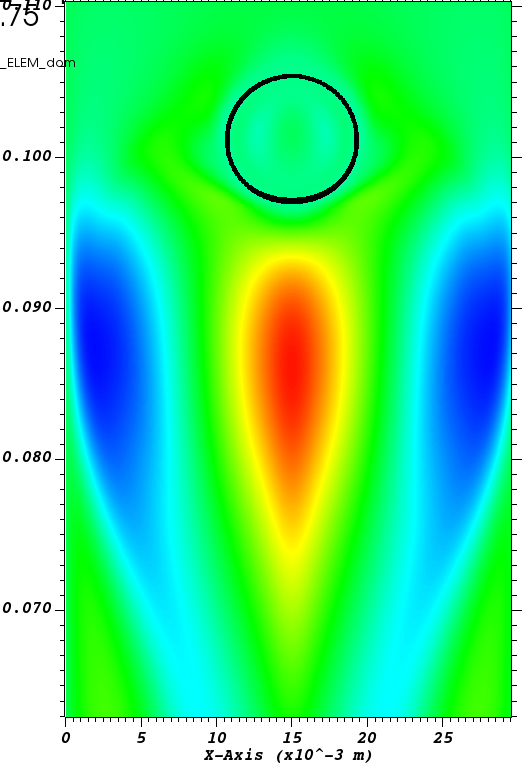
\includegraphics[width=1\textwidth]{fig_plateau_vitesse/visit0009.png}
		\caption{$t=4,75s$}
		\label{fig:three sin x}
	\end{subfigure} 
	\begin{subfigure}[ht!]{0.23\textwidth}
		\centering
		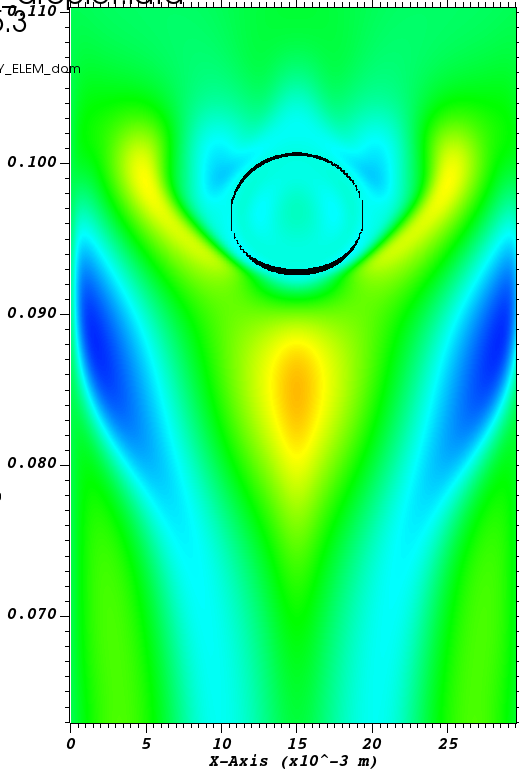
\includegraphics[width=1\textwidth]{fig_plateau_vitesse/visit0013.png}
		\caption{$t=5,3s$}
		\label{fig:three sin x}
	\end{subfigure}
	\begin{subfigure}[ht!]{0.23\textwidth}
		\centering
		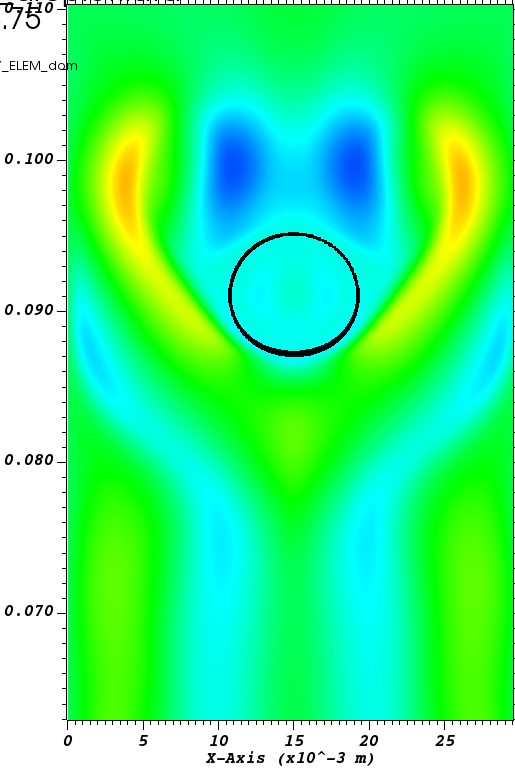
\includegraphics[width=1\textwidth]{fig_plateau_vitesse/visit0016.png}
		\caption{$t=5,75s$}
		\label{fig:three sin x}
	\end{subfigure}
	\begin{subfigure}[ht!]{0.23\textwidth}
		\centering
		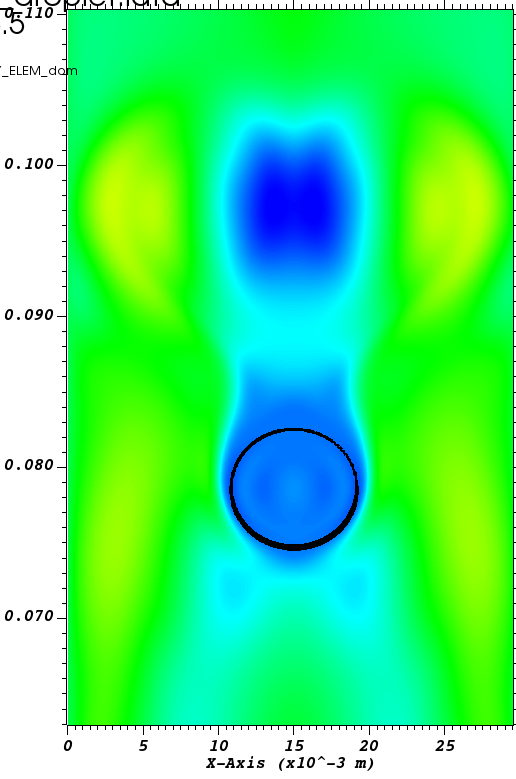
\includegraphics[width=1\textwidth]{fig_plateau_vitesse/visit0019.png}
		\caption{$t=6,5s$}
		\label{fig:three sin x}
	\end{subfigure}
	\begin{subfigure}[ht!]{0.4\textwidth}
	\centering
	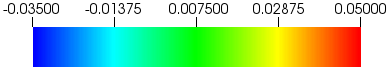
\includegraphics[width=1\textwidth]{fig_plateau_vitesse/colorbar1.png}

\end{subfigure}
	\caption{Champ de vitesses verticales $u_y$ pour une loi de densité linéaire}
	\label{fig:rencotresillage}
\end{figure}
Le second plateau semble également causé par les parois, en effet, il est possible de constater une perturbation du champ de vitesses en Figure \ref{fig:secondplat2}. L'écoulement étant confiné avec des conditions aux limites de type paroi (composante normale et tangentielle de la vitesse nulle aux parois), l'écoulement est fortement dépendant des parois pour un si petit domaine. Un élargissement du domaine est donc étudié en section \ref{sec:tailledom}.  
\begin{figure}[H] 
	\centering
	\begin{subfigure}[ht!]{0.18\textwidth}
		\centering
		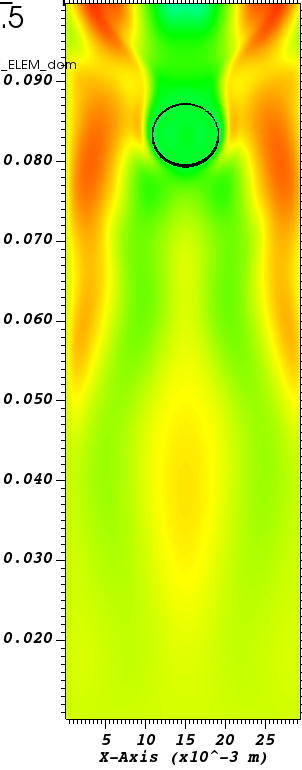
\includegraphics[width=1\textwidth]{fig_plateau_vitesse2/visit0012.png}
		\caption{$t=6,5s$}
	\end{subfigure}
	\begin{subfigure}[ht!]{0.18\textwidth}
		\centering
		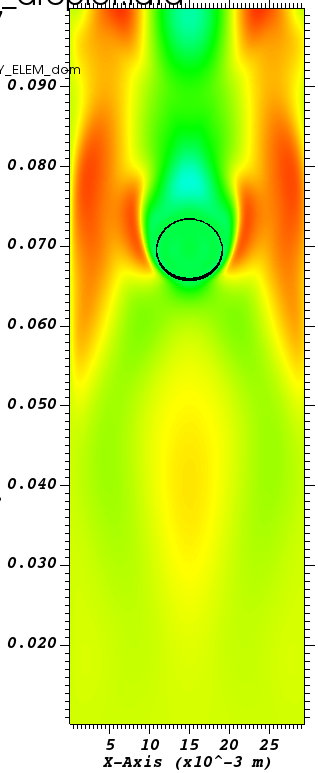
\includegraphics[width=1\textwidth]{fig_plateau_vitesse2/visit0014.png}
		\caption{$t=7s$}
	\end{subfigure}
	\begin{subfigure}[ht!]{0.18\textwidth}
		\centering
		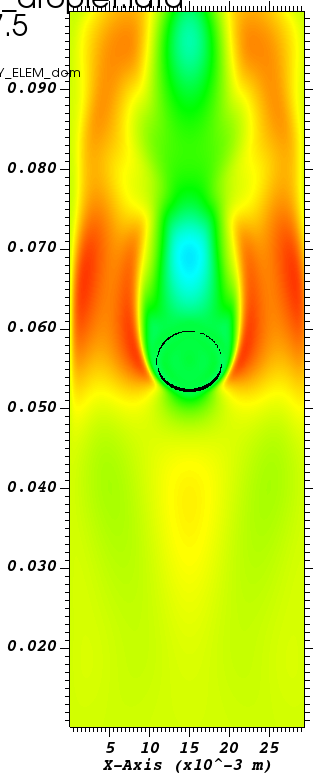
\includegraphics[width=1\textwidth]{fig_plateau_vitesse2/visit0016.png}
		\caption{$t=7,5s$}
	\end{subfigure}
	\begin{subfigure}[ht!]{0.18\textwidth}
		\centering
		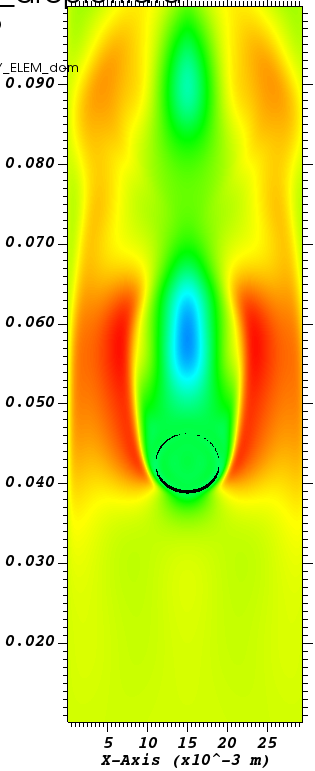
\includegraphics[width=1\textwidth]{fig_plateau_vitesse2/visit0018.png}
		\caption{$t=8s$}
	\end{subfigure}
	\begin{subfigure}[ht!]{0.18\textwidth}
		\centering
		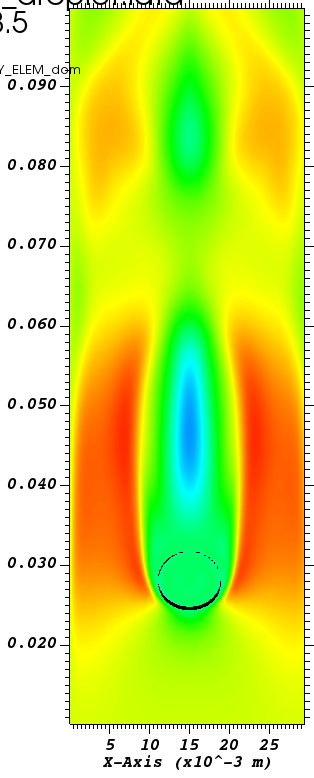
\includegraphics[width=1\textwidth]{fig_plateau_vitesse2/visit0020.png}
		\caption{$t=8,5s$}
	\end{subfigure}
	\begin{subfigure}[ht!]{0.4\textwidth}
	\centering
	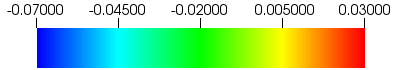
\includegraphics[width=1\textwidth]{fig_plateau_vitesse2/colorbar2.png}
\end{subfigure}
	\caption{Champ de vitesses verticales $u_y$ pour une loi de densité linéaire}
	\label{fig:secondplat2}
\end{figure}

\subsection{Sensibilité des résultats au choix du paysage thermodynamique}
Le paysage étant déterminé de façon arbitraire, dans cette section nous cherchons à comparer les résultats relatifs à deux paysages pour démontrer l'impossibilité à réaliser des simulations quantitatives sans bases thermodynamiques liée au système. Ainsi, nous comparons deux paysages présentés en Figure \ref{fig:comparelandscape} (notés paysage a et b, le paysage a étant le paysage utilisé dans les simulations précédentes). Les deux paysages respectent les critères énoncés en section \ref{subsec:critere_admi} et possèdent les mêmes comportements aux temps longs. Les paramètres des simulations modifiés par rapport au tableau \ref{table:cas_ref} sont présentés dans le tableau \ref{table:newlandscape}. Le choix de la mobilité pour le paysage b a été réalisé suivant les mêmes critères, en choisissant la mobilité qui permet d'obtenir le temps de retour à la hauteur de départ équivalent.
\begin{figure}[H]
	\centering
	\begin{subfigure}[H]{0.45\textwidth}
		\centering
		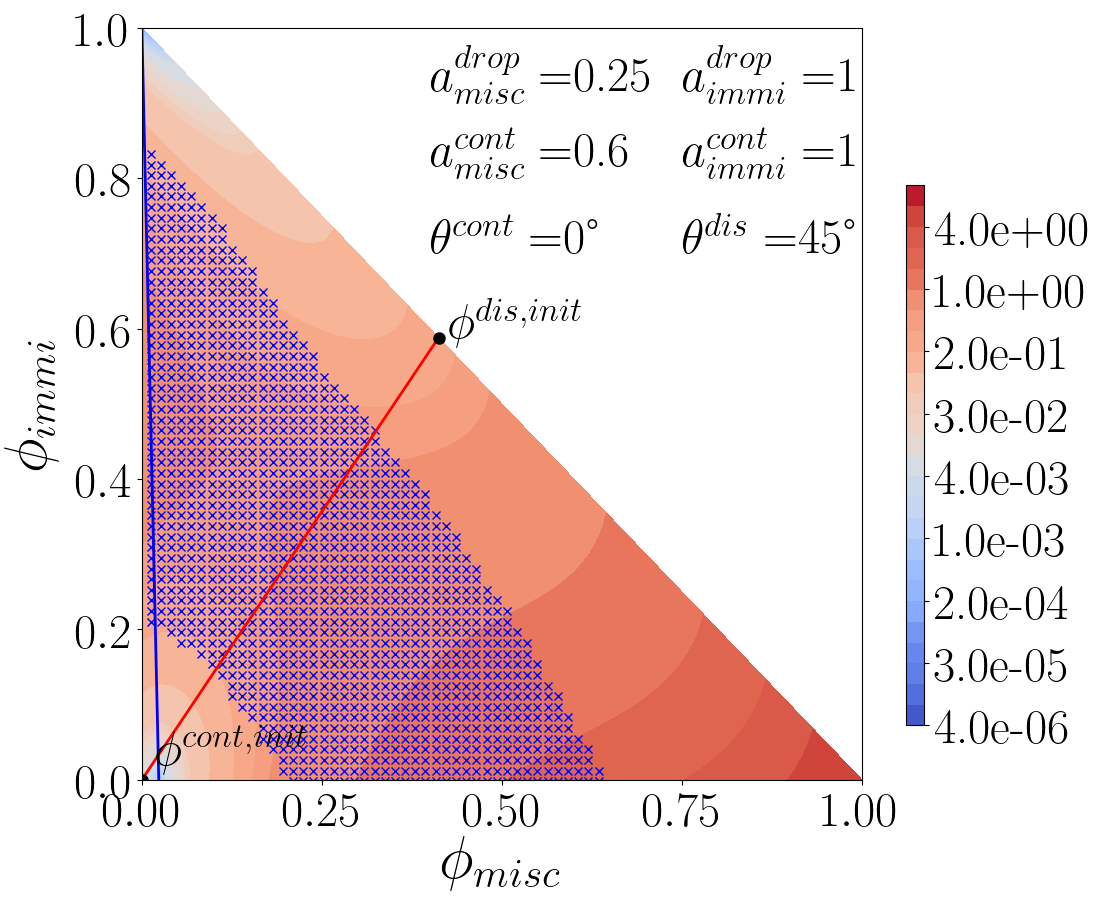
\includegraphics[width=1.1\textwidth]{figure/Paysage_ecriture1.png}
		\caption{Paysage a}
		\label{fig:paysage1}
	\end{subfigure}
	\hfill
	\begin{subfigure}[H]{0.45\textwidth}
		\centering
		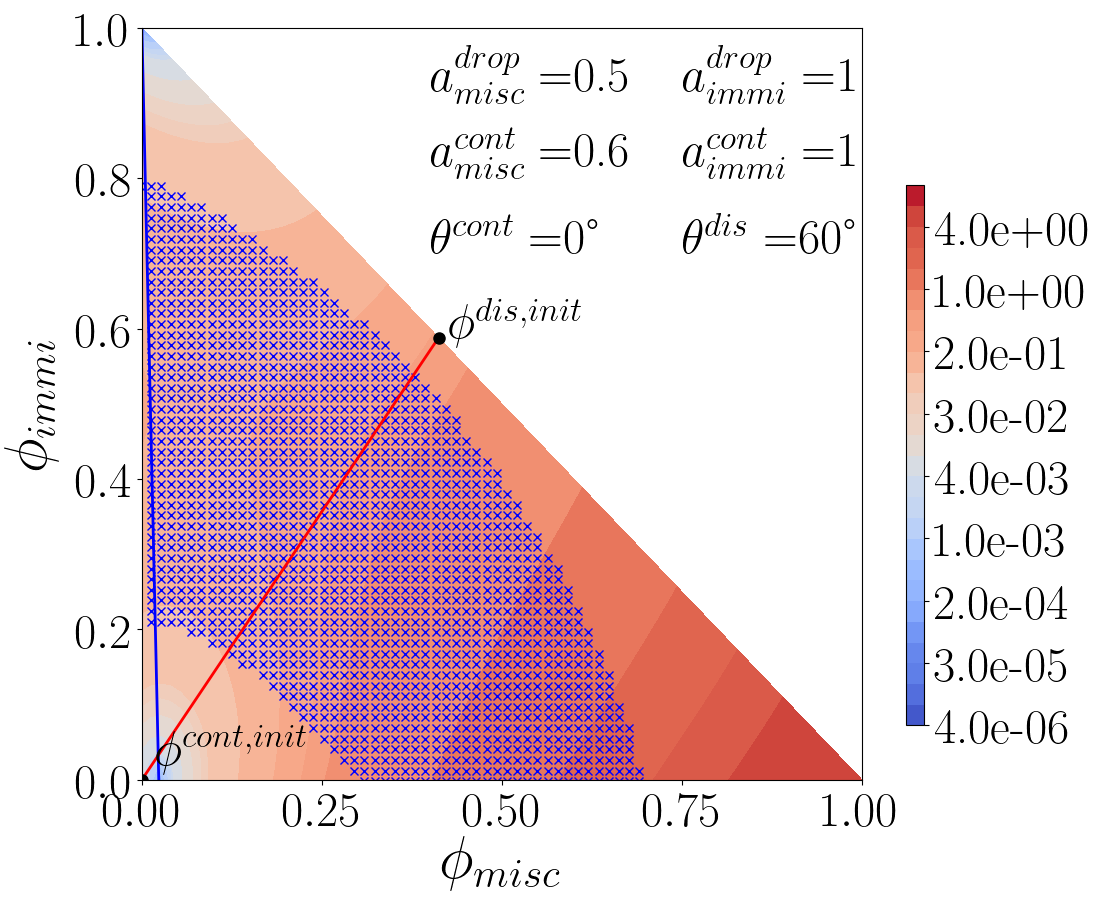
\includegraphics[width=1.1\textwidth]{figure/paysagetocompare.png}
		\caption{Paysage b}
		\label{fig:paysage2}
	\end{subfigure}
	\caption{Paysages thermodynamique utilisés pour la comparaison, la sous-Figure \ref{fig:paysage1} représente le paysage choisit jusqu’à présent et est donc identique à la figure \ref{fig:thechoosenone}}
	\label{fig:comparelandscape}
\end{figure}
\begin{table}[H]
	\centering  % not needed, since table is as wide as text block
	\begin{tabularx}{\textwidth}{@{}lYYYY@{}}
		\toprule
		
		&\multicolumn{3}{c}{\bfseries Paramètres "champ de phase"}\\
		%\cmidrule(lr){2-3} \cmidrule(l){4-5} 
		& $\lambda$ (-)
		& $\kappa$
		& $\mathcal{M}$ (m$^2$.s$^{-1}$)\\
		\midrule
		\textcolor{blue}{Paysage de référence}  & \textcolor{blue}{22,87} & 4,32.10$^{-5}$ $\delta_{ij}$ & \textcolor{blue}{4.10$^{-9}$} $\delta_{ij}$ \\
		\textcolor{orange}{Nouveau paysage }  & \textcolor{orange}{111,08} & 4,32.10$^{-5}$ $\delta_{ij}$ & \textcolor{orange}{5.10$^{-10}$} $\delta_{ij}$ \\
		\bottomrule
	\end{tabularx}
	\caption{Paramètres de simulation} \label{table:newlandscape}
\end{table}
Les résultats de position et de vitesse de la goutte sont présentés en Figure \ref{fig:impactpaysage}.
\begin{figure}[H] 
	\centering
	\begin{subfigure}[H]{0.47\textwidth}
		\centering
		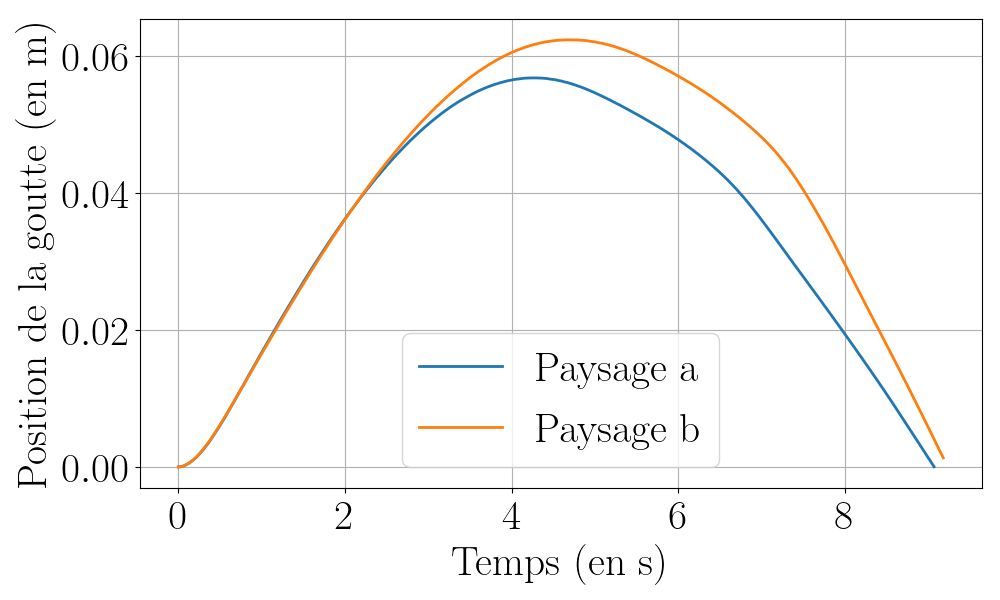
\includegraphics[width=\textwidth]{figure/influence_Landscape_position.png}
		\caption{Trajectoire de la goutte}
	\end{subfigure} 
	\begin{subfigure}[H]{0.47\textwidth}
		\centering
		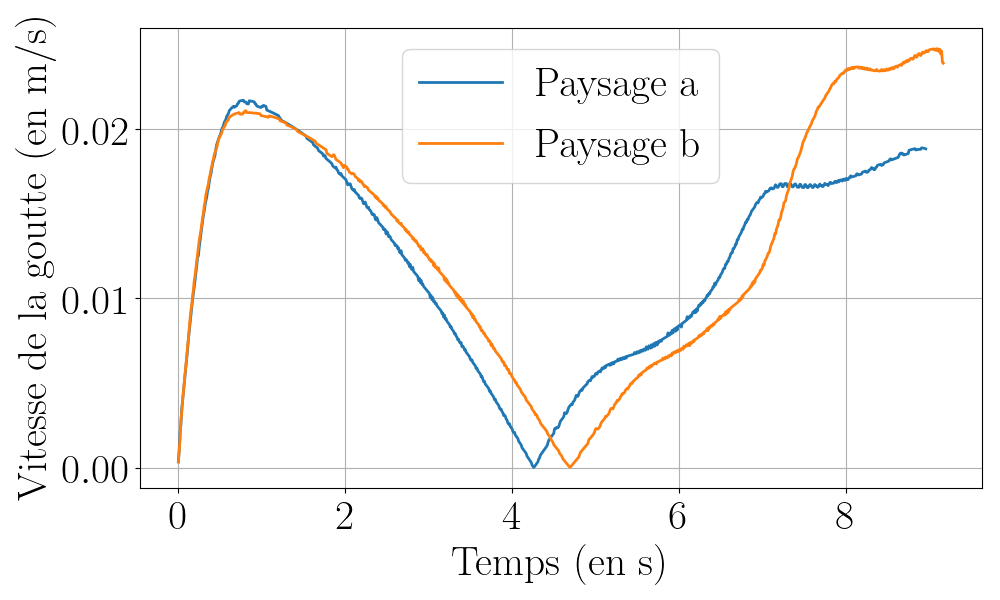
\includegraphics[width=\textwidth]{figure/influence_Landscape_vitesse.png}
		\caption{Vitesse de la goutte}
	\end{subfigure}
	\caption{Trajectoire et vitesse de la goutte pour deux paysages différents}
	\label{fig:impactpaysage}
\end{figure}
Sur ces figures, il est possible de remarquer qu'après 6s un important écart apparaît entre les vitesses selon le paysage. Pour comprendre cet écart, la somme des concentrations et les masses volumiques sont tracées en Figure \ref{fig:otherland_sommeConcent}. On y remarque que la contrainte sur la somme des concentrations n'est pas respectée pour le paysage b, ainsi la goutte contient 12,9\% de matière supplémentaire non-physique tandis que le paysage a n'en contient que 2\%. Il est également possible de remarque, au travers du panache présent dans le champ de masses volumiques du paysage b, que le paysage b diffuse bien plus d'élément miscible que le paysage a. Ainsi, on peut déduire que la goutte s'alourdit plus vite dans ce second cas favorisant une accélération et une vitesse plus importante.
\begin{figure}[H] 
	\centering
	\begin{subfigure}[H]{0.47\textwidth}
		\centering
		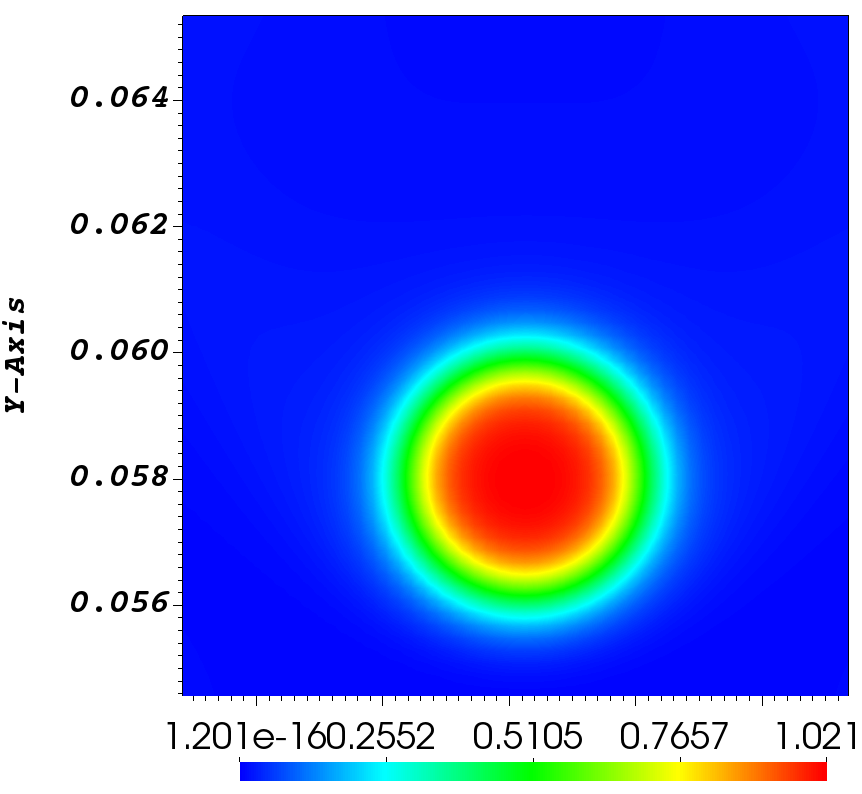
\includegraphics[width=\textwidth]{figure/somme_concentration_a_6s.png}
		\caption{Somme des concentrations, paysage a}
	\end{subfigure} 
	\begin{subfigure}[H]{0.47\textwidth}
		\centering
		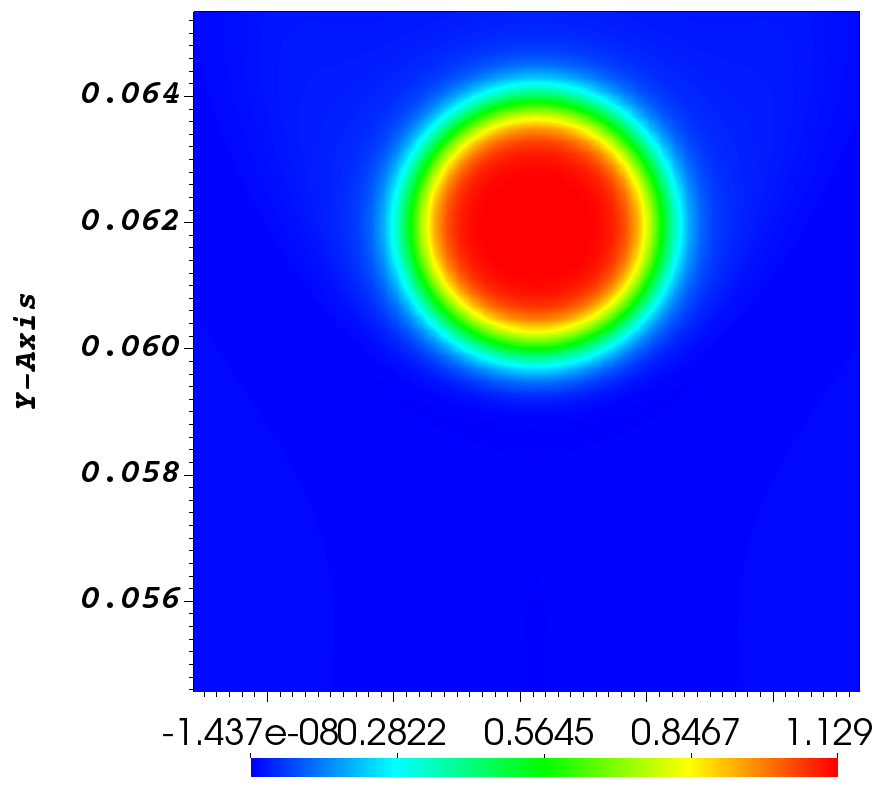
\includegraphics[width=1.05\textwidth]{figure/somme_concentration_other_6s.png}
		\caption{Somme des concentrations, paysage b}
	\end{subfigure}
	\begin{subfigure}[H]{0.47\textwidth}
	\centering
	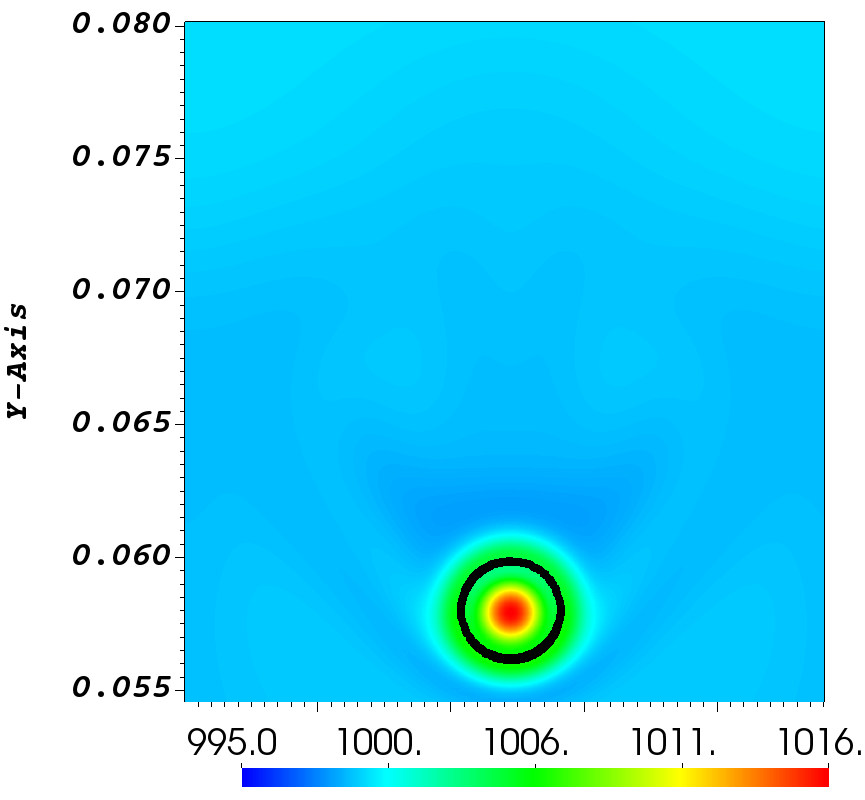
\includegraphics[width=\textwidth]{figure/masse_vol_a_6s.png}
	\caption{Masse volumique, paysage a}
\end{subfigure} 
\begin{subfigure}[H]{0.47\textwidth}
	\centering
	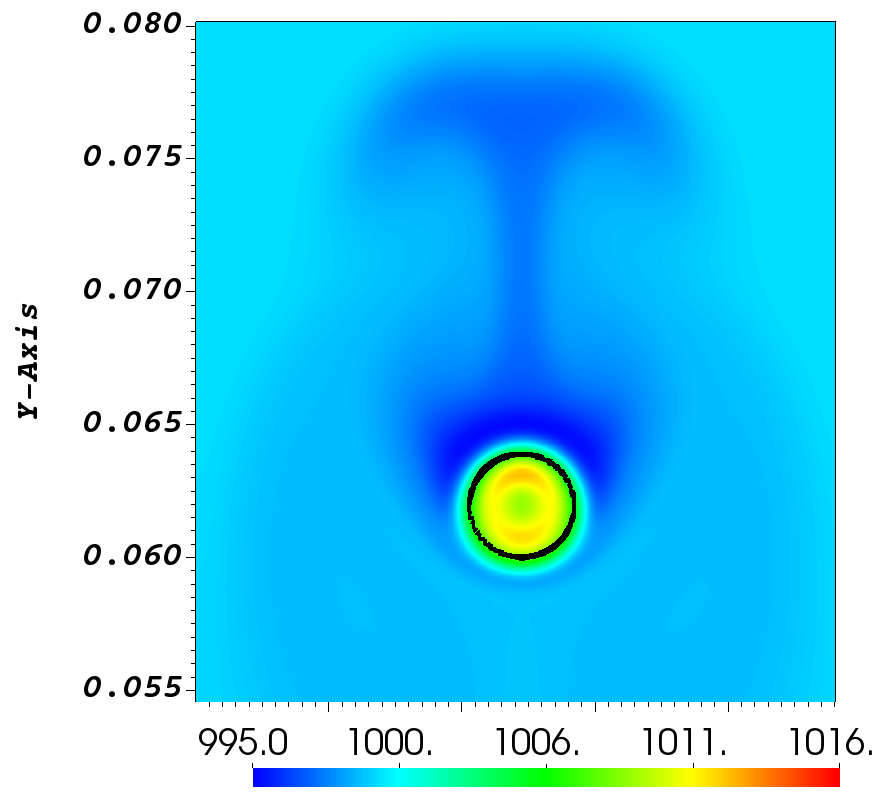
\includegraphics[width=\textwidth]{figure/masse_vol_other_6s.png}
	\caption{Masse volumique, paysage b}
\end{subfigure}
	\caption{Somme des concentrations miscible et immiscible à t=6s}
	\label{fig:otherland_sommeConcent}
\end{figure}
Finalement, nous avons montré que le choix du paysage pouvait grandement influer sur les résultats obtenus. De plus, nous avons pu observer que ce second paysage ne respecte pas les contraintes physiques liées au paramètre d'ordre. Ainsi, pour la suite de ce travail, nous utiliserons le paysage a.

\subsection{Ajout d'un champ de vitesses initial}
Comme expliqué en section \ref{sec:presExp}, il existe une forte incertitude sur les conditions initiales de l'expérience et notamment sur la vitesse initiale de goutte, les relevés des positions étant commencés 1s après la formation de la goutte. Ainsi pour nous rapprocher des résultats fournit par Rao et al. \cite{rao_influence_2015}, nous proposons d'initialiser un champ de vitesse. Ainsi, dans le jeu de données, la condition initiale de vitesse s'écrit :
\begin{subequations}
	\begin{empheq}[left={\empheqlbrace\,}]{align}
	&u_x(\mathbf{x},t=0) = 0\\
	&u_y(\mathbf{x},t=0) = C + C\tanh\left(\cfrac{\sqrt{(x-x_0)^2+(y-y_0)^2}-R}{\epsilon} \right)
	\end{empheq}
\end{subequations}
Avec $C$ une constante dépendante de la valeur de vitesse souhaitée. Ces conditions initiales de la forme tangente hyperbolique proviennent de la solution analytique de l'état d'équilibre d'un système possédant une interface plane. La condition initiale de vitesse peut être discutée, en effet pour obtenir des conditions réalistes, il serait nécessaire de connaître l'entièreté du champ de vitesses. Cependant, c'est avec ce type de condition initiale que l'on arrive le mieux à retranscrire une vitesse initiale de la goutte. Cependant il est important de noter que les équations de Navier-Stokes sont résolues en utilisant une méthode de projection, ainsi la condition initiale de vitesse fournit dans le jeu de données n'est pas la condition initiale utilisée par TrioCFD, la Figure \ref{fig:champvitesse_init} représente les champs de vitesses initiales pour $C=0.05$. Les résultats associés à ce champ de vitesses initiales et à un champ de vitesses initiales nulles sont présentés en Figure \ref{fig:resultat_vitesse}. \\
\begin{figure}[H] \label{fig:champvitesse_init}
	\centering
	\begin{subfigure}[H]{0.47\textwidth}
		\centering
		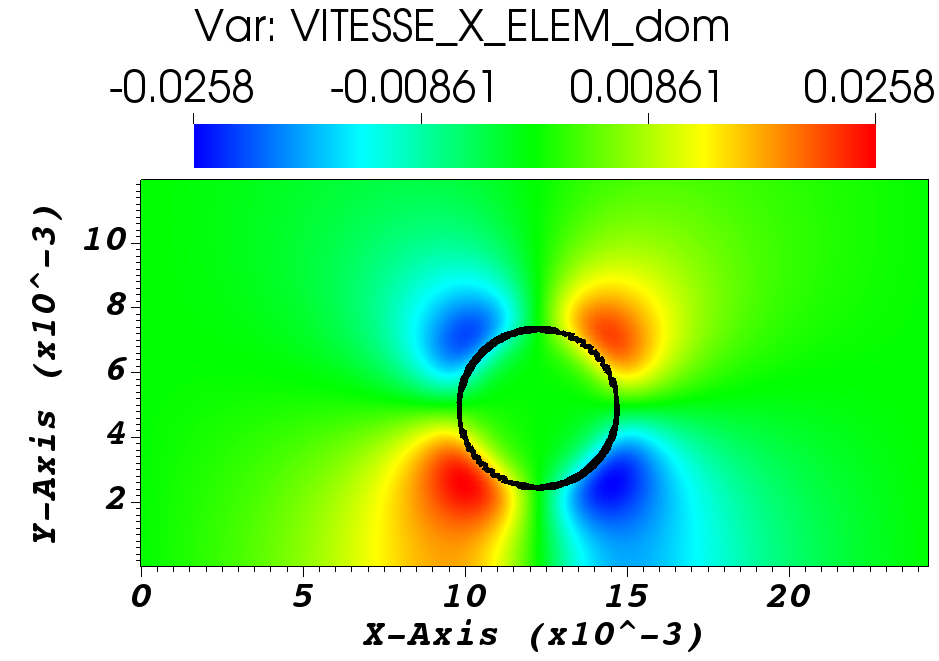
\includegraphics[width=\textwidth]{figure/Champ_vitesse_initX.png}
		\caption{Champ de vitesses horizontales $u_x$}
		
	\end{subfigure} 
	\begin{subfigure}[H]{0.47\textwidth}
		\centering
		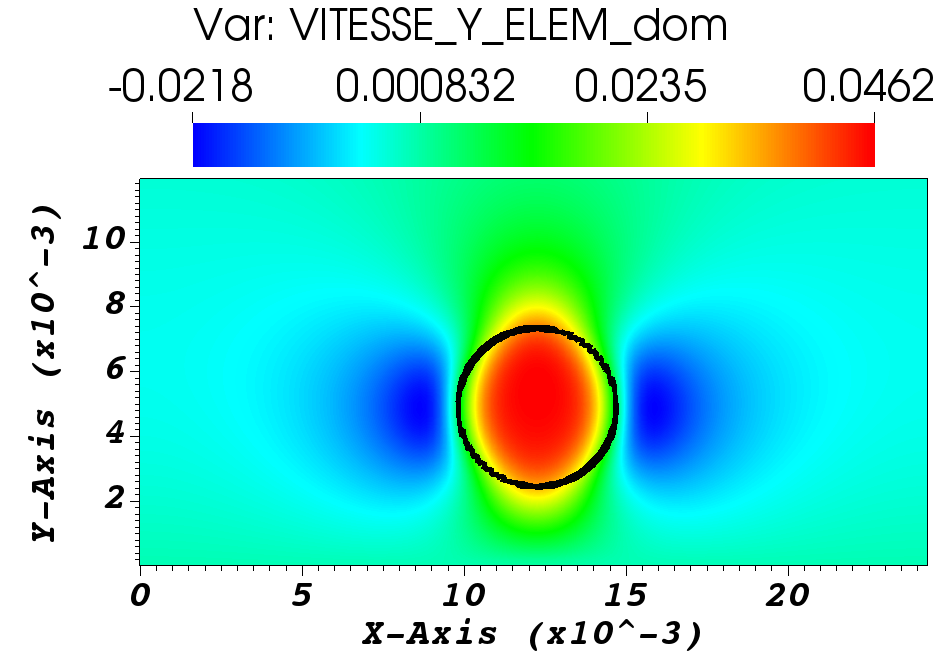
\includegraphics[width=\textwidth]{figure/Champ_vitesse_initY.png}
		\caption{Champ de vitesses verticales $u_y$}
	\end{subfigure}
	\caption{Champ de vitesses initial après projection}
\end{figure}
\begin{figure}[H] \label{fig:resultat_vitesse}
	\centering
	\begin{subfigure}[H]{0.47\textwidth}
		\centering
		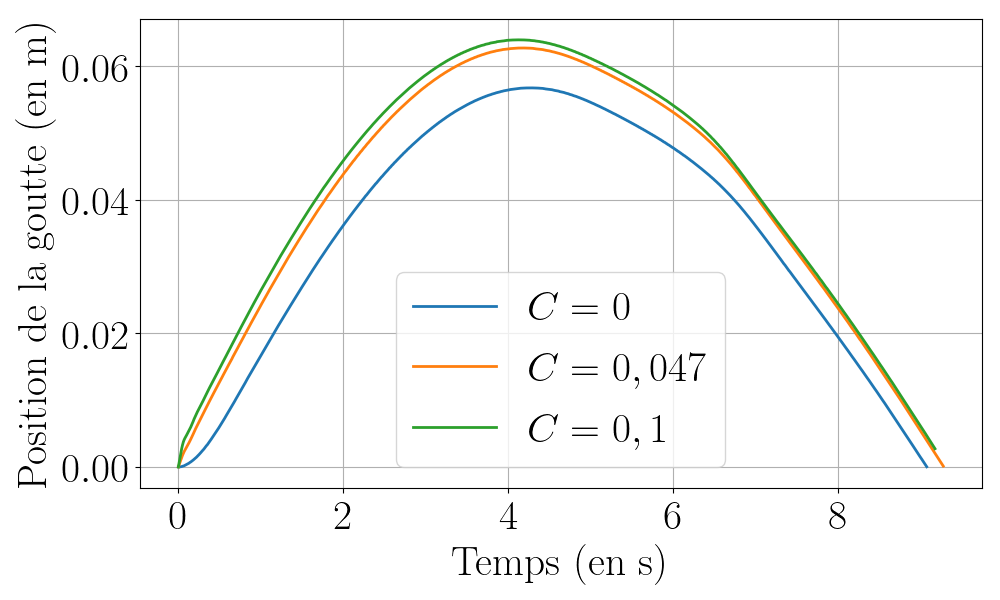
\includegraphics[width=\textwidth]{figure/influence_uinit_position.png}
		\caption{Trajectoire de la goutte}
		
	\end{subfigure} 
	\begin{subfigure}[H]{0.47\textwidth}
		\centering
		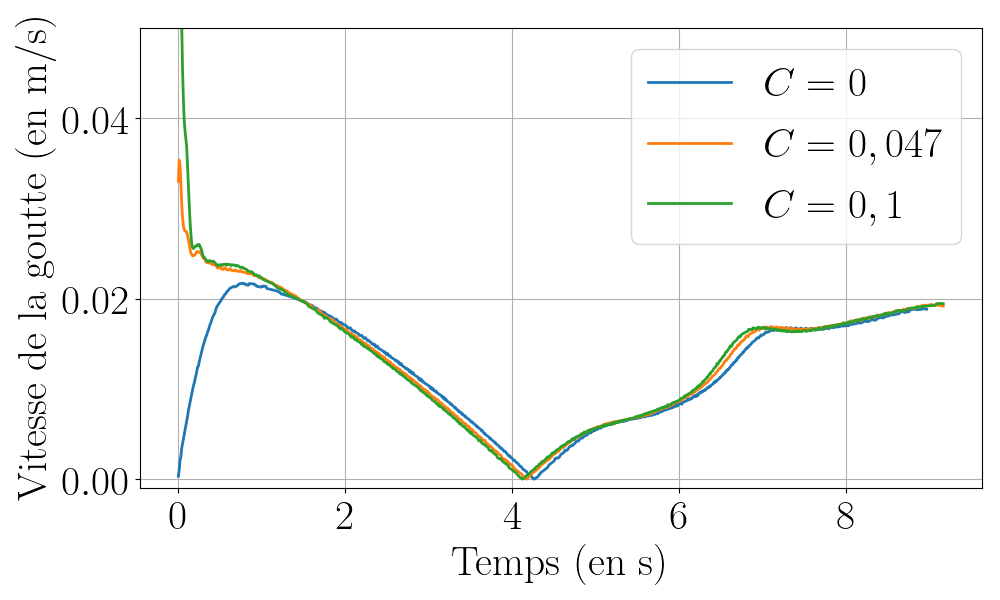
\includegraphics[width=\textwidth]{figure/influence_uinit_vitesse.png}
		\caption{Vitesse de la goutte}
	\end{subfigure}
	\caption{Trajectoire et vitesse de la goutte pour une vitesse initiale nulle (bleu) et non-nulle (orange et vert)}
\end{figure}
On remarque alors que pour des temps supérieurs à t=1,5s, la vitesse de la goutte n'est quasiment plus influencée par la condition initiale de vitesse, les instants d'inversion étant sensiblement identiques (un écart inférieur à 0,25s), il en va de même sur la phase descendante ou les résultats semblent identiques. Ainsi, l'ajout d'une condition initiale de vitesse ne semble pas pertinent et nous nous limiterons à des conditions initiales de vitesses nulles pour la suite.


\subsection{Modification de la loi de densité}
Nous avons pu voir précédemment que l'amplitude de trajectoire de la goutte était réduite par rapport à l'expérience proposée par Rao et al.. L'amplitude étant pilotée par le terme de flottabilité dans l'équation de Navier-Stokes, le choix de la loi de densité est très important vis-à-vis des résultats. Ainsi, nous proposons de modifier la loi de densité pour se rapprocher des conditions expérimentales. Cette nouvelle loi de densité est construite de sorte à pouvoir conserver l'ensemble des conditions initiales (masse volumique des corps purs et de la goutte ainsi que les conditions initiales dans la goutte) soient satisfaites dans nos simulations. Cette loi est notée $\rho^{mix}$ (en opposition à $\rho^{lin}$ la loi précédemment utilisée présentée en équation \ref{eq:boussi}) et s'écrit sous la forme :
\begin{equation*}
\rho^{mix}({\phi_{misc},\phi_{immi}}) = \rho_{eau} \left(   1 + \beta_{misc}\phi_{misc} +\beta_{immi} \phi_{immi} + \beta_{mix}\phi_{misc}\phi_{immi} \right)
\end{equation*} \vspace{-1cm}
\begin{figure}[H]
	\centering
	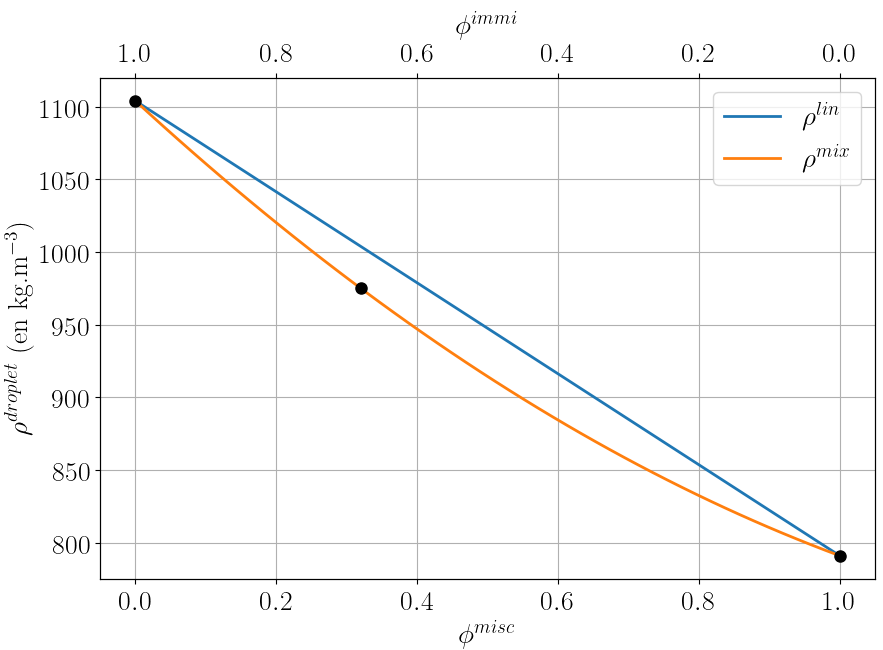
\includegraphics[width=0.65\linewidth]{figure/rho_droplet}
	\label{fig:rhodroplet}
	\caption{Loi de densité dans la goutte sans intrusion d'eau, les points noirs représentent les données fournies par Rao et al. \cite{rao_influence_2015}}
\end{figure}
Le coefficient de dilation associé au terme non linéaire $\beta_{mix}$ se calcul tel que :
\begin{equation}
	\beta_{mix} = \frac{1}{\phi_{misc}^{init,disp}\phi_{immi}^{init,disp}} \left(\frac{\rho^{init,disp}}{\rho_{eau}}- 1 - \beta_{misc} \phi_{misc}^{init,disp} - \beta_{immi} \phi_{immi}^{init,disp}\right)
\end{equation}
Avec $\phi_{misc}^{init,disp}$ (resp. $\phi_{immi}^{init,disp}$) la valeur de concentration initiale de l'élément miscible (resp. immiscible) dans la goutte d'après Rao et al. \cite{rao_influence_2015}.\\
Cette loi de densité va à l'encontre de l'hypothèse du volume molaire constant. En effet, si le volume molaire est constant alors la densité doit être une combinaison linéaire des densités des corps purs. Les paramètres relatifs aux simulations comparant deux lois de densité sont présentés dans le Tableau \ref{table:rhomix}, les résultats de trajectoire et de vitesse sont, quant à eux, tracés en Figure \ref{fig:resultat_rhomix}

\begin{table}[H]
	
	\centering  % not needed, since table is as wide as text block
	\begin{tabularx}{\textwidth}{@{}lYYYYYYY@{}}
		\toprule
		&\multicolumn{7}{c}{\bfseries Paramètres physiques}\\
		%\cmidrule(lr){2-3} \cmidrule(l){4-5} 
		& $\rho^*$ (kg.m$^{-3}$)
		& $\eta$ (Pa.s)
		& $\beta_{misc}$ (-)
		& $\beta_{immi}$ (-)
		& $\beta_{mix}$ (-)
		& $\epsilon$ (m)
		& $\sigma$ (N.m$^{-1}$)\\
		\midrule
		\textcolor{blue}{Cas $\rho^{lin}$} & 999,5 & 10$^{-3}$& -0,21 & 0,10 &  \textcolor{blue}{$\emptyset$}& 8.10$^{-4}$ & 36.10$^{-3}$ \\
		\textcolor{orange}{Cas $\rho^{mix}$} & 999,5 & 10$^{-3}$& -0,21 & 0,10 & \textcolor{orange}{-0,13}  & 8.10$^{-4}$ & 36.10$^{-3}$ \\
		\bottomrule
	\end{tabularx}
	\begin{tabularx}{\textwidth}{@{}lYYYYYYYY@{}}
		\toprule
		&\multicolumn{8}{c}{\bfseries Conditions initiales et d'équilibres}\\
		%\cmidrule(lr){2-3} \cmidrule(l){4-5} 
		& $\phi_{misc}^{drop}$ 
		& $\phi_{immi}^{drop}$ 
		& $\phi_{misc}^{cont}$ 
		& $\phi_{immi}^{cont}$
		& $\phi_{misc}^{drop,eq}$ 
		& $\phi_{immi}^{drop,eq}$ 
		& $\phi_{misc}^{cont,eq}$ 
		& $\phi_{immi}^{cont,eq}$ \\
		\midrule
		\textcolor{blue}{Cas $\rho^{lin}$}  & \textcolor{blue}{0,42} &\textcolor{blue}{0,58} & 0 & 0 & 0 & 1 & \textcolor{blue}{2,1.10$^{-3}$ }& 0\\
		\textcolor{orange}{Cas $\rho^{mix}$}  & \textcolor{orange}{0,32} & \textcolor{orange}{0,68} & 0 & 0 & 0 & 1 & \textcolor{orange}{1,6.10$^{-3}$} & 0 \\
		\bottomrule
	\end{tabularx}
	\caption{Paramètres de simulation pour différentes lois de densité, en couleurs les modifications par rapport au tableau \ref{table:cas_ref}} \label{table:rhomix}
\end{table}


\begin{figure}[H] 
	\centering
	\begin{subfigure}[H]{0.47\textwidth}
		\centering
		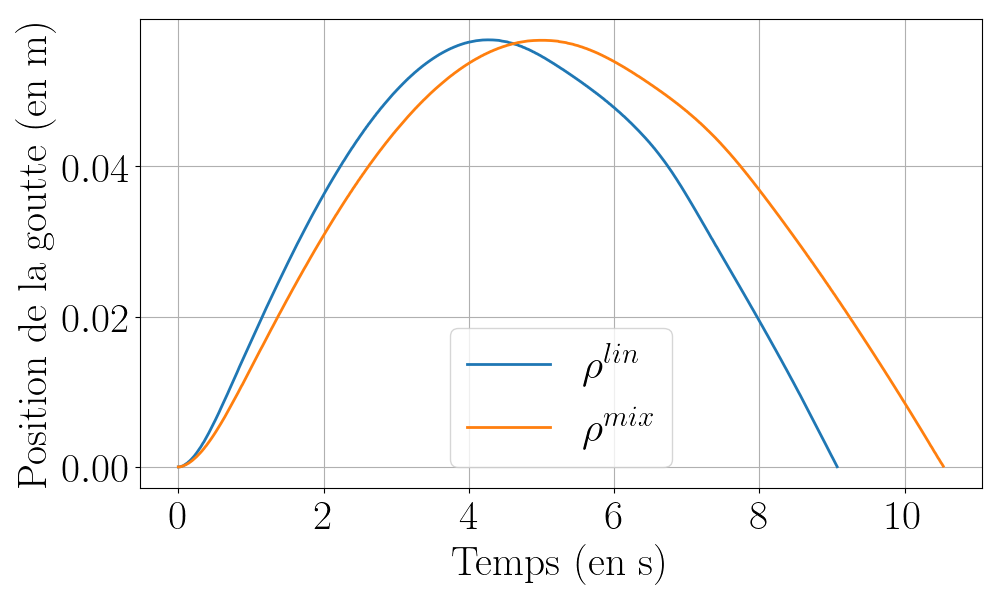
\includegraphics[width=\textwidth]{figure/influence_DensityLaw_position.png}
		\caption{Trajectoire de la goutte}

	\end{subfigure} 
	\begin{subfigure}[H]{0.47\textwidth}
		\centering
		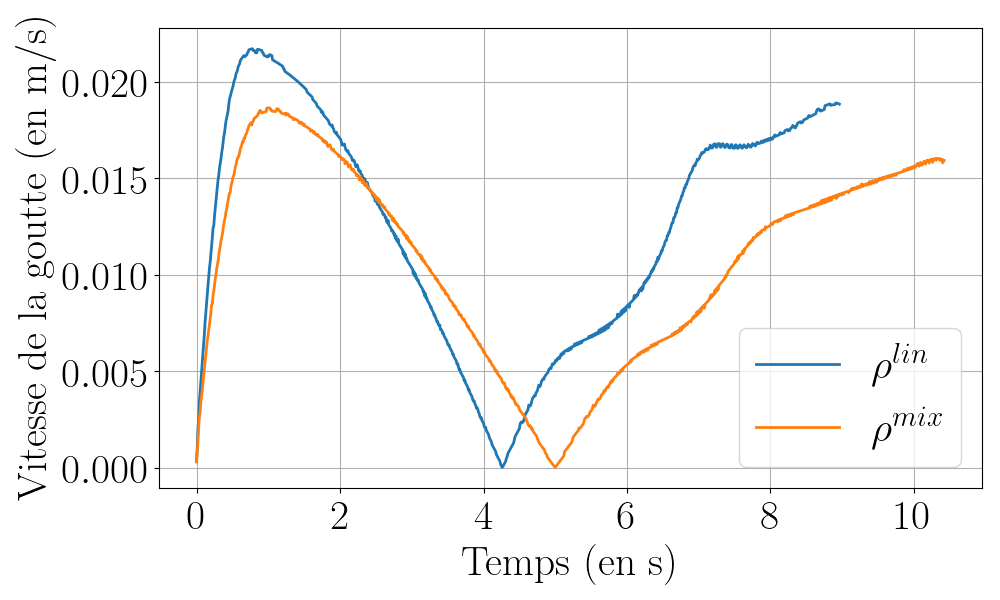
\includegraphics[width=\textwidth]{figure/influence_DensityLaw_vitesse.png}
		\caption{Vitesse de la goutte}
	\end{subfigure}
	\caption{Trajectoire et vitesse de la goutte pour différentes lois de densité}
	\label{fig:resultat_rhomix}
\end{figure}
Ces résultats montrent que la modification de la loi de densité ne permet pas d'obtenir de meilleurs résultats, en effet les vitesses maximales atteinte par la goutte pour les phases ascendante et descendante sont plus faible pour une loi de densité linéaire. Ainsi, le temps terminal (temps pour lequel la goutte est à une hauteur nulle) est supérieur et ne correspond plus à l'expérience. Pour se rapprocher de l'expérience, en supposant que les conclusions faites en section \ref{sec:calibmo} sont transposables avec notre nouvelle loi de densité, la mobilité devrait être augmentée. Cependant augmenter la mobilité réduit la hauteur maximale atteinte par la goutte. Ainsi, cette nouvelle loi de densité ne sera plus considérée pour la suite de ce travail.



\subsection{Modification des conditions aux limites de parois}
Nous avons vu précédemment que la taille du domaine pouvait avoir un impact négatif sur les résultats. Pour limiter l'impact du domaine une des solutions est de négliger l'influence de la couche limite. Pour cela, nous utilisons, sur les parois latérales du domaine une condition aux limites dites de Knudsen non-négligeable. Cette condition s'écrit pour un écoulement isotherme :
\begin{subequations}
	\begin{empheq}[left={\empheqlbrace\,}]{align}
	&u_n = 0\\
	&u_{\tau} - u_{wall} = k \left.\frac{\partial u_{\tau}}{\partial x_n} \right|_{wall}
	\end{empheq}
\end{subequations}
Avec $u_n$ (resp. $x_n$) la composante normale à la paroi de la vitesse (resp. position), $u_{\tau}$ la composante tangentielle de la vitesse par rapport à la paroi, $u_{wall}$ la vitesse de glissement de la paroi et $k$ un coefficient décrivant le régime du fluide (au sens de la continuité). Dans le cas où $k=0$ la condition revient à une condition de paroi fixe comme celle utilisée précédemment, dans le cas où $k\rightarrow+\infty$, la condition aux limites traduit une condition de non-glissement à la paroi, la vitesse tangentielle n'est alors plus fonction de la vitesse de la paroi. Ainsi, dans notre cas, cela revient à négliger la couche limite sur les parois latérales. Les résultats de position de vitesse de la goutte pour différentes valeurs de $k$ sont présentés en Figure \ref{fig:resultat_knudsen}.

\begin{figure}[H] 
	\centering
	\begin{subfigure}[H]{0.47\textwidth}
		\centering
		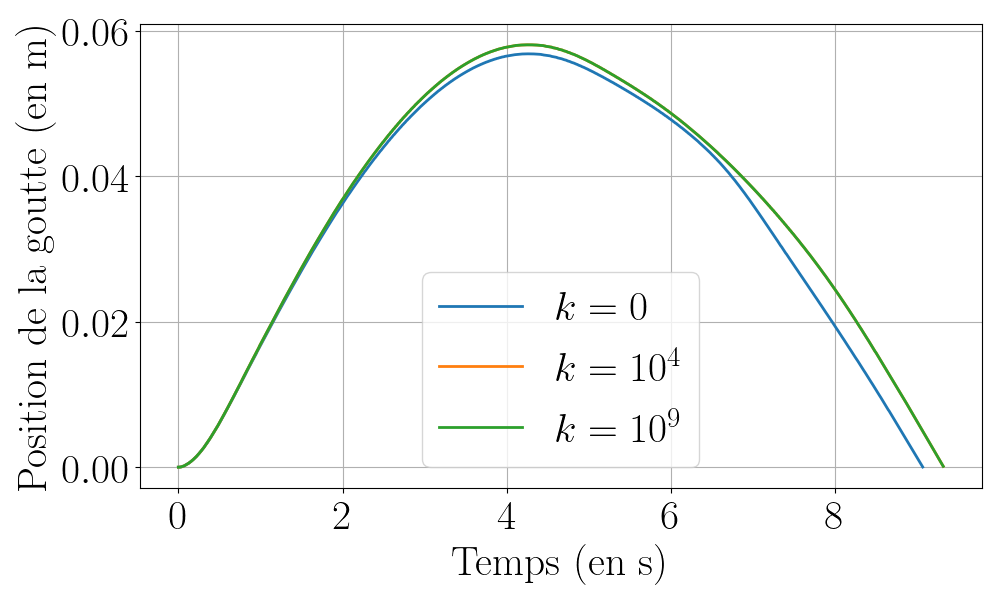
\includegraphics[width=\textwidth]{figure/knudsen_influence_k_position.png}
		\caption{Trajectoire de la goutte}
		
	\end{subfigure} 
	\begin{subfigure}[H]{0.47\textwidth}
		\centering
		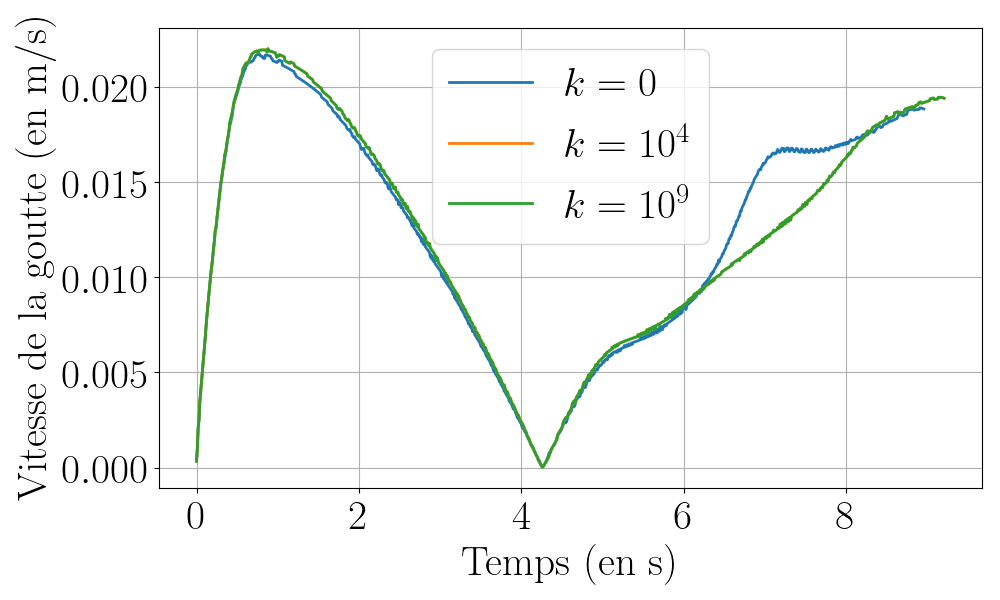
\includegraphics[width=\textwidth]{figure/knudsen_influence_k_vitesse.png}
		\caption{Vitesse de la goutte}
	\end{subfigure}
	\caption{Trajectoire et vitesse de la goutte pour différentes valeurs de $k$ (les courbes $k=10^4$ et $10^9$ sont superposées)}
	\label{fig:resultat_knudsen}
\end{figure}
Il est alors possible d'observer que les résultats sont quasiment identiques sur la phase ascendante, c'est uniquement pour 6,5s<t<8s que la vitesse de la goutte est différente. Pour essayer de comprendre cet écart, le champ des vitesses verticales à différents instants est tracé en Figure \ref{fig:champvitesse_knud}. On y observe que dans le cas où la couche limite est négligée, le sillage de la goutte formé pendant la phase descendante se détache plus tard, en effet on observe que la vitesse nulle aux parois favorise le décrochage dans le cas d'une paroi fixe.
\begin{figure}[H]
	\centering
	\begin{subfigure}[ht!]{0.3\textwidth}
		\centering
		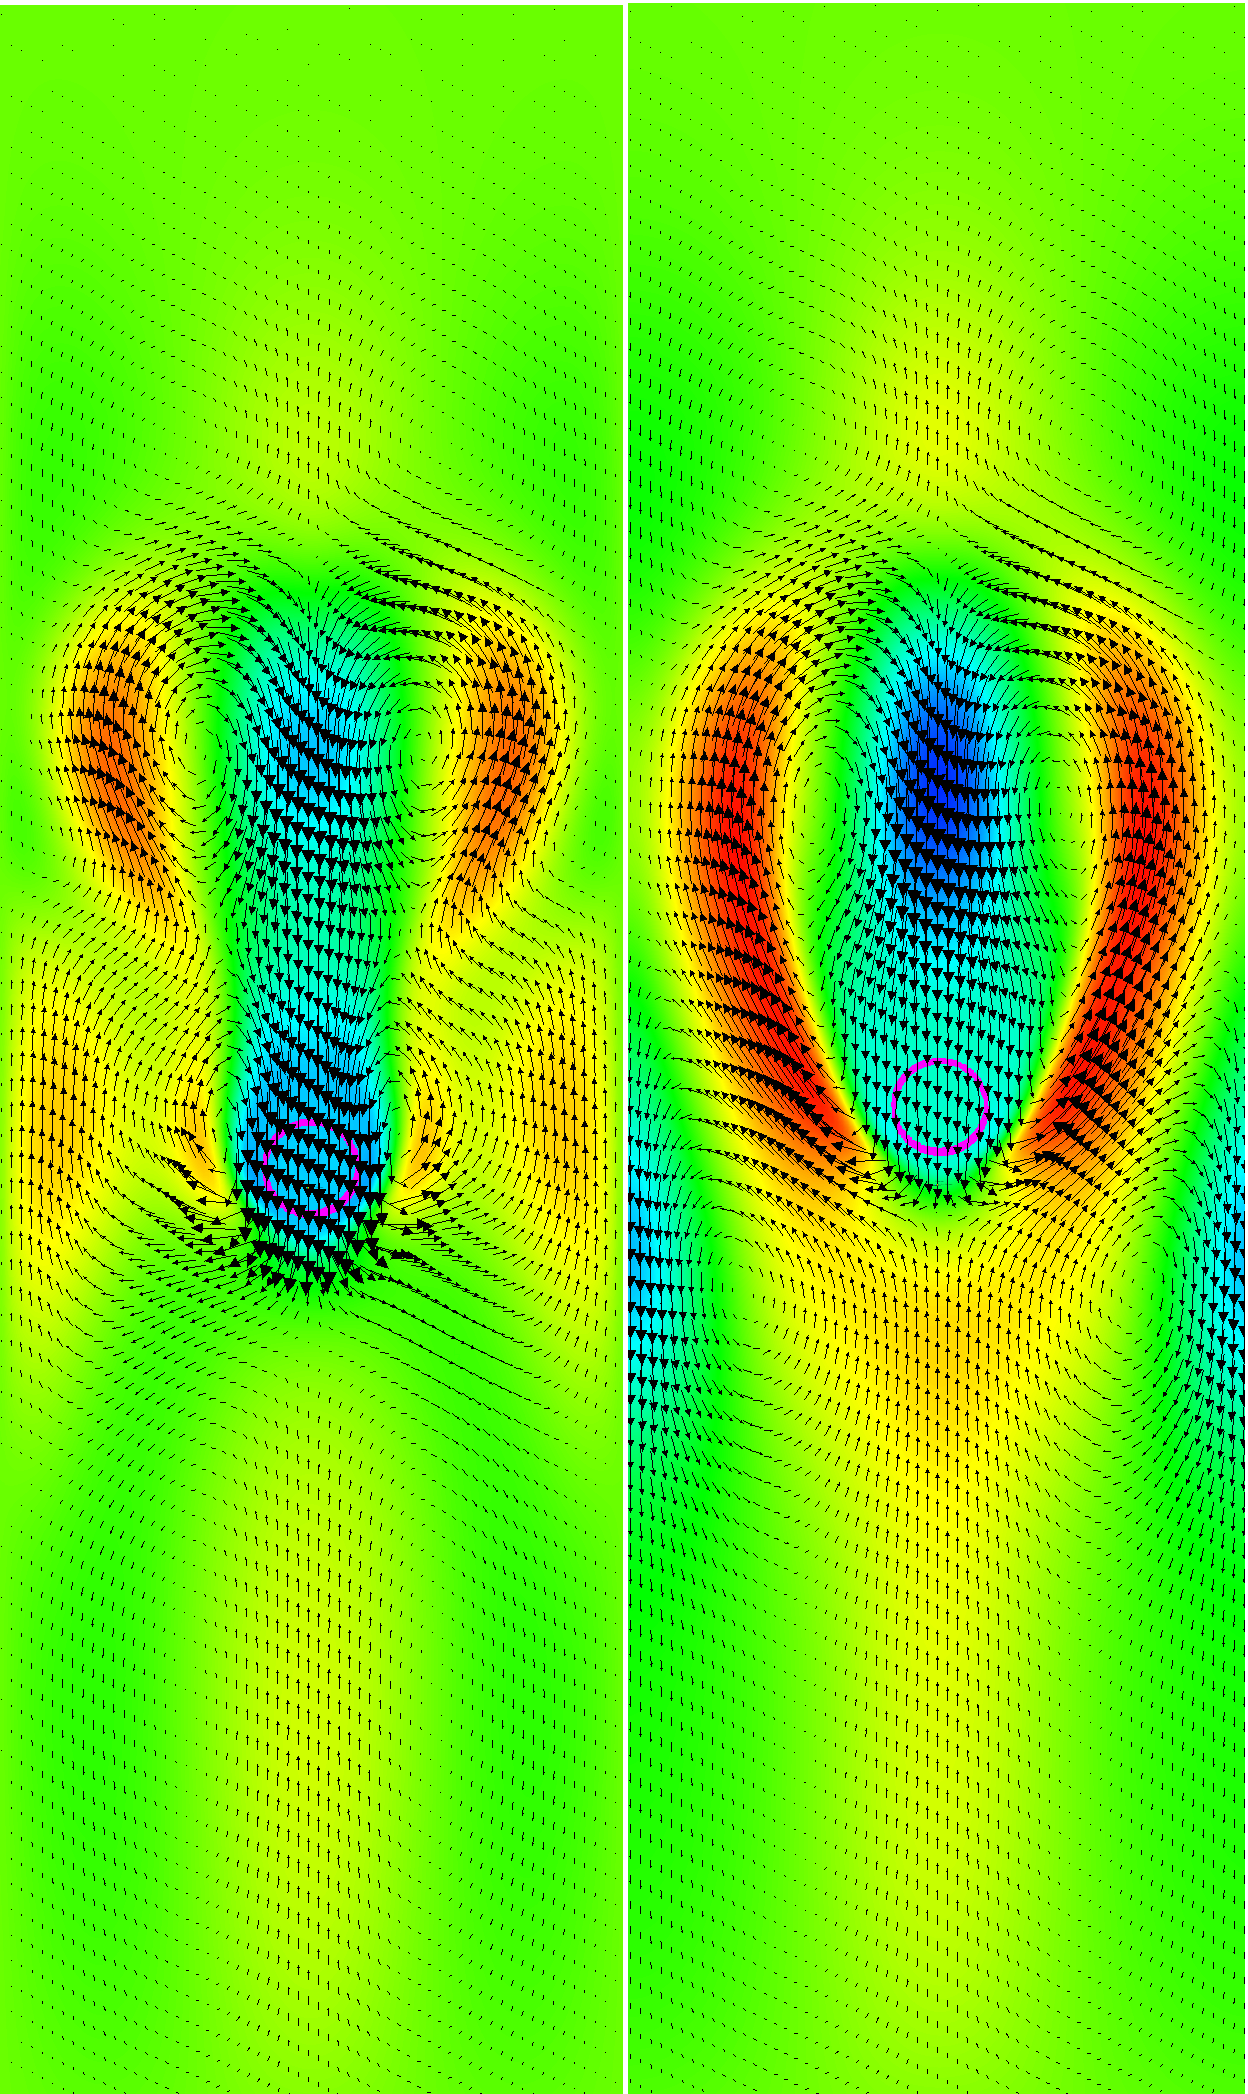
\includegraphics[width=1\textwidth]{compare_CL/t=7s.png}
		\caption{$t=7s$}
	\end{subfigure}
	\begin{subfigure}[ht!]{0.3\textwidth}
		\centering
		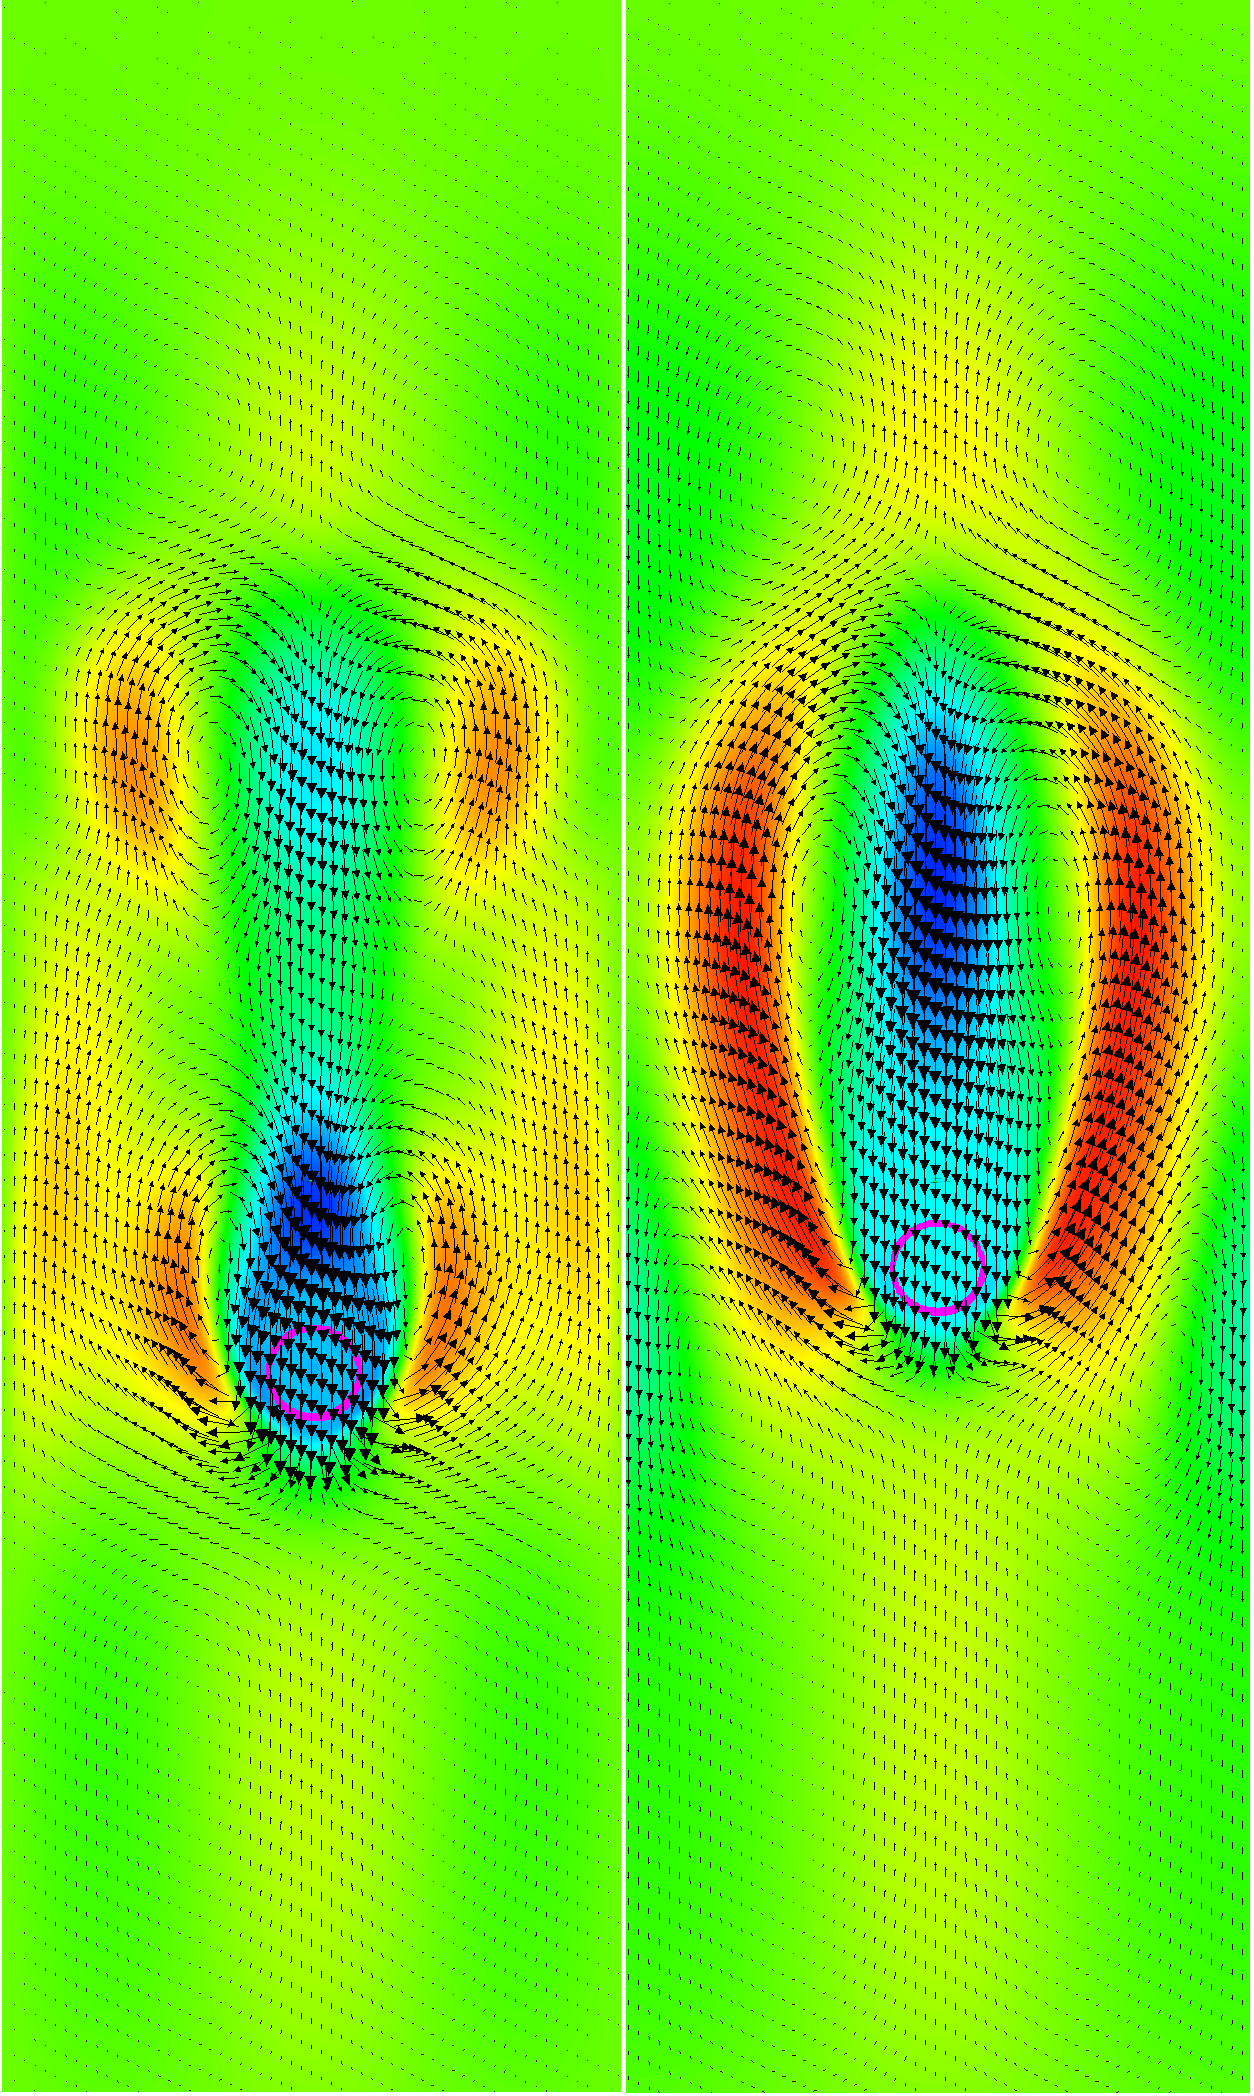
\includegraphics[width=1\textwidth]{compare_CL/t=7,5s.png}
		\caption{$t=7,5s$}
	\end{subfigure}
	\begin{subfigure}[ht!]{0.3\textwidth}
		\centering
		\includegraphics[width=1\textwidth]{compare_CL/t=8s.png}
		\caption{$t=8s$}
	\end{subfigure}
\end{figure} \vspace{-0.8cm}
\begin{figure}[H]
	\centering
	\ContinuedFloat
	\begin{subfigure}[ht!]{0.3\textwidth}
		\centering
		\includegraphics[width=1\textwidth]{compare_CL/t=8,5s.png}
		\caption{$t=8,5s$}
	\end{subfigure}
	\begin{subfigure}[ht!]{0.3\textwidth}
		\centering
		\includegraphics[width=1\textwidth]{compare_CL/t=9s.png}
		\caption{$t=9s$}
	\end{subfigure}
\end{figure}\vspace{-0.7cm}
\begin{figure}[H]
	\centering
	\ContinuedFloat
	\begin{subfigure}[ht!]{0.5\textwidth}
		\centering
		\includegraphics[width=1\textwidth]{compare_CL/colorbar.png}
	\end{subfigure}
	\caption{Champ des vitesses verticales pour différents instants, à gauche dans le cas d'une paroi fixe (i.e. $k=0$), à droite dans le cas d'une vitesse tangentielle à la paroi non perturbée ($k=10^{9}$), en fuchsia les contours de la goutte}
	\label{fig:champvitesse_knud}
\end{figure}





\subsection{Influence de la taille du domaine} \label{sec:tailledom}
Nous avons pu observer que la taille du domaine pouvait avoir un effet non-négligeable sur les résultats, confinant la goutte et son champ de vitesse. On cherche donc à quantifier l'impact de la taille du domaine sur les résultats des simulations. L'augmentation de la taille du domaine augmente grandement le temps de calcul, environ 2 à 3 semaines pour un domaine de largeur $L_x = 20R$ contre quelques jours pour un domaine de largeur $L_x = 10R$. Le récapitulatif des paramètres utilisés pour les simulations est présenté en Tableau \ref{table:tailleDom}, les résultats sont quant à eux présentés en Figure \ref{fig:impactdom}.


\begin{table}[H]
	
	\centering  % not needed, since table is as wide as text block
	\begin{tabularx}{\textwidth}{@{}lYYYYYY@{}}
		\toprule
		&\multicolumn{6}{c}{\bfseries Géométrie et maillage}\\
		%\cmidrule(lr){2-3} \cmidrule(l){4-5} 
		& $L_x$ (m)
		& $L_y$ (m)
		& $dx, dy$ (m)
		& $N_x$
		& $N_y$
		& $D^{drop}$  (m)\\
		\midrule
		\textcolor{blue}{Cas $L_x = 10R$}  & \textcolor{blue}{2,45.10$^{-2}$} & 15.10$^{-2}$ & 2.10$^{-4}$ & \textcolor{blue}{123} & 750 & 4,9.10$^{-3}$ \\
		\textcolor{orange}{Cas $L_x = 15R$}  & \textcolor{orange}{3,675.10$^{-2}$} & 15.10$^{-2}$ & 2.10$^{-4}$ & \textcolor{orange}{184} & 750 & 4,9.10$^{-3}$ \\
		\textcolor{green}{Cas $L_x = 20R$}  & \textcolor{green}{4,9.10$^{-2}$} & 15.10$^{-2}$ & 2.10$^{-4}$ & \textcolor{green}{245} & 750 & 4,9.10$^{-3}$ \\
		\bottomrule
	\end{tabularx}
	\begin{tabularx}{\textwidth}{@{}lYYYYYYYY@{}}
		\toprule
		&\multicolumn{8}{c}{\bfseries Conditions initiales et d'équilibres}\\
		%\cmidrule(lr){2-3} \cmidrule(l){4-5} 
		& $\phi_{misc}^{drop}$ 
		& $\phi_{immi}^{drop}$ 
		& $\phi_{misc}^{cont}$ 
		& $\phi_{immi}^{cont}$
		& $\phi_{misc}^{drop,eq}$ 
		& $\phi_{immi}^{drop,eq}$ 
		& $\phi_{misc}^{cont,eq}$ 
		& $\phi_{immi}^{cont,eq}$ \\
		\midrule
		\textcolor{blue}{Cas $L_x = 10R$} &\textcolor{black}{0,42}  &\textcolor{black}{0,58}  & 0 & 0 & 0 & 1 & \textcolor{blue}{2,1.10$^{-3}$} & 0\\
		\textcolor{orange}{Cas $L_x = 15R$}  &0,42  &\textcolor{black}{0,58}  & 0 & 0 & 0 & 1 & \textcolor{orange}{1,4.10$^{-3}$} & 0\\
				\textcolor{green}{Cas $L_x = 20R$}  &0,42  &\textcolor{black}{0,58}  & 0 & 0 & 0 & 1 & \textcolor{green}{1,1.10$^{-3}$} & 0\\
		\bottomrule
	\end{tabularx}
	\caption{Paramètres de simulation, en couleurs les modifications par rapport au tableau \ref{table:cas_ref}} \label{table:tailleDom}
\end{table}

\begin{figure}[H] 
	\centering
	\begin{subfigure}[H]{0.47\textwidth}
		\centering
		\includegraphics[width=\textwidth]{figure/impactDom_nospeed_position.png}
		\caption{Trajectoire de la goutte}
	\end{subfigure} 
	\begin{subfigure}[H]{0.47\textwidth}
		\centering
		\includegraphics[width=\textwidth]{figure/impactDom_nospeed_vitesse.png}
		\caption{Vitesse de la goutte}
	\end{subfigure}
	\caption{Trajectoire et vitesse de la goutte pour différentes largeurs de domaine}
	\label{fig:impactdom}
\end{figure}

Au regard des résultats, il est possible de dire que la goutte était également perturbée sur la phase ascendante. En effet, la vitesse de la goutte est plus importante lors de son ascension pour un domaine plus large. De plus, il est possible de constater que la perturbation liée à la rencontre de la goutte avec son sillage est plus faible, l'écoulement étant moins confiné. Le domaine de calcul utilisé dans Rao et al. \cite{rao_influence_2015} est encore bien plus grand que ceux proposé dans cette étude, il est donc possible de s'imaginer qu'un domaine encore plus grand soit nécessaire pour reproduire au mieux les résultats de l'expérience. On remarque également que l'agrandissement du domaine augmente le temps terminal, ainsi, il serait nécessaire de recalibrer la mobilité pour obtenir des résultats plus cohérents.

\subsection{Influence d'un raffinement du maillage} \label{sec:raffinement}
Pour terminer cette étude paramétrique, nous essayons de quantifier l'erreur liée à la non-convergence de notre maillage. Dans cette section, nous allons donc observer l'impact d'un raffinement du maillage ainsi que l'impact d'un raffinement du maillage et de l'interface. La Figure \ref{fig:influencemesh} présente trajectoires et vitesses obtenues pour différents maillages et différentes épaisseurs d'interfaces.
Lorsque l'épaisseur d'interface est modifiée, on cherche à conserver le terme diffusion dans l'équation de Cahn-Hilliard, cette conservation se traduit par :
\begin{equation} \label{eq:conservationflux}
\sum_{j=1}^{n-1}{\mathcal{M}_{ij}} \nabla\tilde{\mu}_j = \text{cste} \hspace{1cm} \forall \epsilon
\end{equation}
L'équation \ref{eq:conservationflux} induit la condition :
\begin{equation}
	\overline{ \mathcal{M}}_{ij} = \lambda \mathcal{M}_{ij} = \text{cste} \hspace{1cm} \forall \epsilon
\end{equation}
Avec $\overline{ \mathcal{M}}_{ij}$ une mobilité modifiée invariante selon la paramétrisation géométrique. Les paramètres des simulations associées sont présentés dans le Tableau \ref{table:influenceMesh}.


\begin{table}[H]
	\centering  % not needed, since table is as wide as text block
	\begin{tabularx}{\textwidth}{@{}lYYYYYY@{}}
		\toprule
		&\multicolumn{6}{c}{\bfseries Géométrie et maillage}\\
		%\cmidrule(lr){2-3} \cmidrule(l){4-5} 
		& $L_x$ (m)
		& $L_y$ (m)
		& $dx, dy$ (m)
		& $N_x$
		& $N_y$
		& $D^{drop}$  (m)\\
		\midrule
		\textcolor{blue}{Cas bleu}  & 2,45.10$^{-2}$ & 15.10$^{-2}$ & \textcolor{blue}{2.10$^{-4}$} & \textcolor{blue}{123} & \textcolor{blue}{750} & 4,9.10$^{-3}$ \\
		\textcolor{orange}{Cas orange}  & 2,45.10$^{-2}$ & 15.10$^{-2}$ & \textcolor{orange}{1,33.10$^{-4}$} & \textcolor{orange}{185} & \textcolor{orange}{1125} & 4,9.10$^{-3}$ \\
		\textcolor{green}{Cas vert}  & 2,45.10$^{-2}$ & 15.10$^{-2}$ & \textcolor{green}{1,33.10$^{-4}$} & \textcolor{green}{185} & \textcolor{green}{1125} & 4,9.10$^{-3}$ \\
	
		\bottomrule
	\end{tabularx}
\end{table} \vspace{-0.8cm}
\begin{table}[H]
	\begin{tabularx}{\textwidth}{@{}lYYYYYY@{}}
		\toprule
		&\multicolumn{6}{c}{\bfseries Paramètres physiques}\\
		%\cmidrule(lr){2-3} \cmidrule(l){4-5} 
		& $\rho^*$ (kg.m$^{-3}$)
		& $\eta$ (Pa.s)
		& $\beta_{misc}$ (-)
		& $\beta_{immi}$ (-)
		& $\epsilon$ (m)
		& $\sigma$ (N.m$^{-1}$)\\
		\midrule
		\textcolor{blue}{Cas bleu} & 999,5 & 10$^{-3}$& -0,21 & 0,10 & \textcolor{blue}{8.10$^{-4}$} & 36.10$^{-3}$ \\
		\textcolor{orange}{Cas orange} & 999,5 & 10$^{-3}$& -0,21 & 0,10 & \textcolor{orange}{8.10$^{-4}$} & 36.10$^{-3}$ \\
		\textcolor{green}{Cas vert} & 999,5 & 10$^{-3}$& -0,21 & 0,10 & \textcolor{green}{5.10$^{-4}$} & 36.10$^{-3}$ \\
		\bottomrule
	\end{tabularx}
\end{table}\vspace{-0.8cm}
\begin{table}[H]
	\begin{tabularx}{\textwidth}{@{}lYYYY@{}}
		\toprule
		&\multicolumn{3}{c}{\bfseries Paramètres "champ de phase"}\\
		%\cmidrule(lr){2-3} \cmidrule(l){4-5} 
		& $\lambda$ (-)
		& $\kappa$
		& $\mathcal{M}$ (m$^2$.s$^{-1}$)\\
		\midrule
		\textcolor{blue}{Cas bleu}  & \textcolor{blue}{22,87.10$^{-5}$} & \textcolor{blue}{4,32.10$^{-5}$} $\delta_{ij}$ & \textcolor{blue}{4.10$^{-9}$}  $\delta_{ij}$ \\	
		\textcolor{orange}{Cas orange}  & \textcolor{orange}{22,87.10$^{-5}$} & \textcolor{orange}{4,32.10$^{-5}$} $\delta_{ij}$ & \textcolor{orange}{4.10$^{-9}$} $\delta_{ij}$ \\
		\textcolor{green}{Cas vert}  & \textcolor{green}{36,59.10$^{-5}$} & \textcolor{green}{2,7.10$^{-5}$} $\delta_{ij}$ & \textcolor{green}{2,5.10$^{-9}$} $\delta_{ij}$ \\
		\bottomrule
	\end{tabularx}
 	\caption{Paramètres des simulations, en couleurs les modifications par rapport au Tableau \ref{table:cas_ref}}
	\label{table:influenceMesh}
\end{table}
\begin{figure}[H] 
	\centering
	\begin{subfigure}[H]{\textwidth}
		\centering
		\includegraphics[width=0.4\textwidth]{figure/legend_modif_epsilon.png}
	\end{subfigure}
\end{figure} \vspace{-0.5cm}
\begin{figure}[H] 
	\centering
	\begin{subfigure}[H]{0.47\textwidth}
		\centering
		\includegraphics[width=\textwidth]{figure/influence_maillage_position.png}
		\caption{Trajectoire de la goutte}
	\end{subfigure} 
	\begin{subfigure}[H]{0.47\textwidth}
		\centering
		\includegraphics[width=\textwidth]{figure/influence_maillage_vitesse.png}
		\caption{Vitesse de la goutte}
	\end{subfigure}
	\caption{Trajectoire et vitesse de la goutte pour différentes résolution de maillage et épaisseur d'interface}
\label{fig:impactmesh}
\end{figure}
Au vu de ces résultats, il est possible de dire que la convergence seule du maillage n'est pas nécessaire ni impactante vis-à-vis des résultats. Cependant, l'amincissement modifie grandement les résultats, les vitesses maximales sur les phases ascendante et descendante sont plus importante tout en conservant la hauteur maximale atteinte. Finalement, la convergence de maillage a un effet non-négligeable. Malgré tout, vu les capacités de calcul disponible, réaliser l'ensemble des calculs convergé en maillage aurait été impossible. Les calculs avec les maillages les plus fin utilisés dans cette étude ont nécessité 3 semaines de calculs. Les résultats non convergé présentant les mêmes tendances, cette étude paramétrique permet tout de même d'obtenir des tendances qui pourront être validées par la suite lorsque les simulations parallèles pourront être menées.

\section{Conclusion sur la comparaison à l'expérience et perspectives d'améliorations}

Au travers de cette étude paramétrique, nous avons pu observer l'influence de divers paramètres sur la trajectoire d'une goutte soumise a de la diffusion massique. Pour permettre de reproduire l'expérience, il faudrait, dans un premier temps avoir la puissance de calcul nécessaire pour réaliser des simulations convergé en espace et en temps pour des domaines que l'on pourrait supposer infini vis-à-vis de la goutte (suffisamment grand pour ne pas impacter sa trajectoire et ses champs de vitesses). De plus, le manque d'information quant au paysage thermodynamique ne nous permettra jamais de réaliser des simulations satisfaisantes au vu de l'incertitude que le choix du paysage représente. Cependant, malgré ses difficultés, nous avons pu mener une étude qualitative sur un nombre important de paramètres permettant une première approche de validation.

